\documentclass[a4paper, twoside, parskip=full]{book}
\usepackage[toc,page]{appendix}
\usepackage{geometry}
\usepackage{makeidx}
\usepackage{graphicx}
\usepackage{tabularx}
\usepackage{multicol}
\usepackage{multirow}
\usepackage{float}
\usepackage{listings}
\usepackage{enumerate}
\usepackage{color}
\usepackage{ifthen}
\usepackage[table]{xcolor}
\usepackage{textcomp}
\usepackage{alltt}
\usepackage{ifpdf}
\ifpdf%
\usepackage[pdftex,
            colorlinks=true,
            linkcolor=blue,
            unicode
           ]{hyperref}
\else
\usepackage[ps2pdf,
            colorlinks=true,
            linkcolor=blue,
            unicode
           ]{hyperref}
\usepackage{pspicture}
\fi
\usepackage[utf8]{inputenc}
\usepackage{mathptmx}
\usepackage[scaled=.90]{helvet}
\usepackage{courier}
\usepackage{parskip}
\usepackage{sectsty}
\usepackage{booktabs}
\usepackage[titles]{tocloft}
\usepackage{fancyhdr}
\usepackage{fancyvrb}
\usepackage{scrextend}
\usepackage{afterpage}
\usepackage[nottoc,numbib]{tocbibind}
\usepackage{pgfplots}
\usepackage{algorithm}
\usepackage{algpseudocode}

\usetikzlibrary{patterns}

\expandafter\def\expandafter\UrlBreaks\expandafter{\UrlBreaks%  save the current one
  \do\a\do\b\do\c\do\d\do\e\do\f\do\g\do\h\do\i\do\j%
  \do\k\do\l\do\m\do\n\do\o\do\p\do\q\do\r\do\s\do\t%
  \do\u\do\v\do\w\do\x\do\y\do\z\do\A\do\B\do\C\do\D%
  \do\E\do\F\do\G\do\H\do\I\do\J\do\K\do\L\do\M\do\N%
  \do\O\do\P\do\Q\do\R\do\S\do\T\do\U\do\V\do\W\do\X%
  \do\Y\do\Z}

\renewcommand{\familydefault}{\sfdefault}

% The geometry of al of our pages
\geometry{
 a4paper,
 total={170mm,237mm},
 left=20mm,
 top=30mm,
}

% Define the thickness of the header and footer rules
\renewcommand{\headrulewidth}{1pt}
\renewcommand{\footrulewidth}{1pt}

% Change the Bibliography name to references
\renewcommand{\bibname}{References}

% A command to provide a completely blank page
\newcommand\blankpage{%
    \null%
    \thispagestyle{empty}%
    \addtocounter{page}{-1}%
    \newpage}

% A method defined in fancyhdr documentation for twosided blank pages before a chapter start
\makeatletter
\def\cleardoublepage{\clearpage\if@twoside\ifodd\c@page\else
  \hbox{}
  \vspace*{\fill}
  \begin{center}
  This page is intentionally left blank.
  \end{center}
  \vspace{\fill}
  \thispagestyle{empty}
  \newpage
  \if@twocolumn\hbox{}\newpage\fi\fi\fi}
\makeatother

% Define the header and footer for all pages except the title and blank pages
\fancypagestyle{plain}{
  \fancyhf{}
  \fancyhead[RE,LO]{SAFEcrypto}
  \fancyhead[LE,RO]{\leftmark}
  \fancyfoot[LE,RO]{\thepage}
}
\pagestyle{plain}

% Configure indexing of the TOC to a depth of 3 levels
\makeindex
\setcounter{tocdepth}{2}

\providecommand{\versionnumber}{1.4}


\begin{document}
\hypersetup{pageanchor=false}

% The title page
\begin{titlepage}
\vspace*{7cm}
\begin{center}
\includegraphics[scale=0.5]{../Resources/SAFEcrypto.png}\\
\vspace*{1cm}
{\Large \textbf{SAFEcrypto}: \textbf{S}ecure \textbf{A}rchitectures of \textbf{F}uture \textbf{E}merging \textbf{Cryptography}}\\
\vspace*{1cm}
{\Huge Software Architecture Document}\\
\vspace*{0.5cm}
{\Large \today}\\
\vspace*{0.5cm}
{\Large Version \versionnumber}\\
\end{center}
\end{titlepage}

% Intentionally leave a blank page after the title/cover page
\afterpage{\blankpage}
\clearpage

% Use Roman numbers for any pages prior to the Introduction
\pagenumbering{roman}

% Insert a Revision History table (MUST BE MANUALLY EDITED)
\begin{table}[ht!]
\centering
\caption{Revision History}
\label{my-label}
\begin{tabularx}{\textwidth}{lll p{10cm}}
\toprule
\textbf{Date} &\textbf{Author} &\textbf{Version}  &\textbf{History}  \\
\midrule
1\textsuperscript{st} Aug 2016 &NS &1.0  &Initial documentation.  \\
\midrule
9\textsuperscript{th} Dec 2016 &NS &1.1  &Updated Architectural View and added an Optimization Appendix. \\
\midrule
9\textsuperscript{th} Feb 2017 &NS &1.2  &Updated diagrams and references. Expanded Architectural View and Optimizations. \\
\midrule
24\textsuperscript{th} March 2017 &NS &1.3  &Updated version number description, added IBE and AKE discussion. \\
\midrule
8\textsuperscript{th} May 2017 &NS &1.4  &Updated Use Case View, Process View and HW integration. Added details to the Appendix. \\
\midrule
 &  &  &  \\
\midrule
 &  &  &  \\
\midrule
 &  &  &  \\
\midrule
 &  &  &  \\
\midrule
 &  &  &  \\
 \bottomrule
\end{tabularx}
\end{table}

% Insert a Table of Contents
\tableofcontents

% From this point onwards insert a blank page WHERE NECESSARY to ensure chapters start on the right
\clearpage{\pagestyle{empty}\cleardoublepage}

% Use Arabic numbering from this point onwards
\pagenumbering{arabic}
\hypersetup{pageanchor=true}


\mainmatter

\chapter{Introduction}
\label{ch_introduction}

This Introduction provides an overview of the entire \textit{Software Coding Guidelines} document for SAFEcrypto.
It includes the purpose, scope, definitions, acronyms, abbreviations, references and a document overview.

\section{Purpose}
SAFEcrypto will provide a new generation of practical, robust, and physically secure post-quantum cryptographic functions. Work Package 6 will develop a suite of software routines to implement the lattice-based constructions identified in Work Package 4 of the SAFEcrypto project.

A well designed system can be rendered useless at the implementation stage if poor coding and weak coding practices are used. All coding environments, no matter how small the project is, must have a set of policies and guidelines that are well documented and enforced. The adoption of a uniform set of rules and guidelines will promote robust coding practices that achieve software assurance.

Coding Standards exist for a range of languages, the Software Engineering Institute (SEI) contains secure coding standards for C, \verb!C++!, Java, Perl and Android and is an excellent resource for information around software assurance. Typically network and systems level code is written in C/\verb!C++! and the reality is a large amount of cryptographic code and security protocols are written in these languages.

While these are some of the most powerful and performance enhancing languages available, they are also amongst the most dangerous. The danger lies in the flexibility of these languages, and that they are at a lower level of compilation. As the level of language compilation gets lower bugs and vulnerabilities become more difficult to detect.

The SEI Secure Coding Standards contain a comprehensive wiki of rules and recommendations:

\begin{enumerate}
	\item Rules provided are normative requirements for code violations have the potential to introduce a security vulnerability and are detectable through code analysers.
	\item Recommendations provide guidance on increasing software assurance at a code level these are not compulsory and are suggestions that can increase the level of assurance within code. Recommendations are typically enforced in accordance with the product requirements, for example high grade security products will normally enforce many of the recommendations. A system that has critical safety requirements may go even further by enforcing safety standards, e.g. a ban on dynamic memory etc.
\end{enumerate}

This document provides a set of secure coding guidelines and principles that will ensure that the software development process adheres to best practices in trustworthy software development. In addition to secure coding guidelines some rules with regards to style guidelines are also provided, this is to provide a consistent and readable source code package that will be released into the public domain. In addition the build system and various build tools are described that will be used to automate the process of rule checking.

\section{Scope}
The scope of this document includes the entire SAFEcrypto software development lifecycle including architecture and design, implementation, build infrastructure and testing strategy. A well-documented and enforceable coding standard is an essential element of coding in the C programming language.

A SAFEcrypto coding standard encourages developers to follow a set of rules that benefit the SAFEcrypto project in terms of producing software that is secure, reliable and robust. These rules can be checked manually (e.g.\ code reviews) or using automated processes incorporated into the build system (e.g. Lint, CppCheck).


\section{Definitions, Acronyms and Abbreviations}
\begin{labeling}{SAFEcrypto}
\item [SAD] Software Architecture Document
\item [SAFEcrypto] Safe Architectures of Future Emerging Cryptography
\item [WP\textit{N}] Work Package \textit{N}
\end{labeling}

\section{References}
The following documents should be read in conjunction with this \textit{Software Architecture Document}:

\begin{itemize}
\item SAFEcrypto: Secure Architectures of Future Emerging Cryptography, H2020-ICT-2014--1~\cite{safecrypto_overview}
\item SAFEcrypto: Software Requirements Specification, Version 1.0, April 22 2016~\cite{safecrypto_srs}
\item SAFEcrypto: Software Architecture Document, Version 1.0,~???
\end{itemize}

\section{Overview}
This document consists of 5 sections which are described below:

\begin{itemize}
\item Section 1 is simply an introduction to the coding guidelines of the SAFEcrypto software system.
\item Section 2 identifies the goals and constraints of the coding guidelines.
\item Section 3 describes an overview of the proposed software system.
\item Section 4 provides a set of rules for C programming language development.
%\item Section 5 discusses the automated tools that will be incorporated into the build system.
%\item Section 6 provides a description of the code review process.
\item Section 5 is a bibliography of the references used to create this document.
\end{itemize}



\chapter{Architectural Goals and Constraints}
\label{ch_goals_and_constraints}

The SAFEcrypto software architecture has been designed with the following objectives in mind:

\begin{itemize}
\item Low overhead lattice-based cryptographic software implementations for embedded platforms.
  \begin{enumerate}[(a)]
  \item Low level cryptographic algorithms optimised for a small memory footprint.
  \item Optimisation of arithmetic intensize operations for high speed implementations.
  \end{enumerate}
\item High performance lattice-based cryptographic software implementations for multi-core architectures:
  \begin{enumerate}[(b)]
  \item A fully pipelined parallel architecture to maximise throughput.
  \item Optimisation of scheduling and resource allocation for high scalability.
  \end{enumerate}
\item Future hardware acceleration using FPGA/ASIC.
\end{itemize}

\vspace{5mm}

\noindent
The major design and implementation constraints on the system are:

\begin{itemize}
\item Portability
\item Reliability
\item Security
\item Maintainability
\item Flexibility
\end{itemize}

\vspace{5mm}

The \textit{libsafecrypto} library must adhere to the security coding guideliness described in \cite{safecrypto_secure_coding_guidelines} and discussed in Chapter \ref{ch_security}.



\chapter{Architectural View Decomposition}
\label{ch_architectural_view}

A system must be viewed from different perspectives in order to model, implement and document that system. Therefore the 4+1 Model View will be used to represent the SAFEcrypto software system: Use Case View, Logical View, Development View, Process View and Physical View.


\begin{itemize}
	\item Use Case View: the main purpose of the Use Case View is to define the system requirements.
	\item Logical View: this view contains system definitions and class diagrams to describe the services that the system will provide to its users.
	\item Development View: this view will provide system and user interface specficiations
	\item Process View: this view will use collaberation, sequence and activity diagrams to describe the processes that form the system.
	\item Physical View: this view will depict how the systems' hardware nodes will interact and how they are installed.
\end{itemize}


\section{Stakeholders}
\label{sec:stakeholders}

The following is a list of stakeholders who are actively involved with the project, are affected by the outcome or have an influence in the development of the SAFEcrypto library.

\begin{itemize}
	\item \textbf{Developer} - responsible for the development of the software.
	\item \textbf{Maintainer} - responsible for enhancement and fixing of the software.
	\item \textbf{Researcher} - utilise the project to implement, analyse and evaluate the cryptographic schemes that they develop.
	\item \textbf{Tester} - responsible for quality assessment of the library to ensure it is robust
	\item \textbf{User} - will use the software directly.
\end{itemize}

\section{Use Case View}
\label{sec_use_case}

This section lists descriptions of the most significant use cases of the software.

\subsection{Cryptographic Operation on a Message}

Figure \ref{fig:use_case_1} shows a User creating an instance of the SAFEcrypto library that provides a specific scheme and uses a defined parameter set. The User either generates a key-pair or loads a private and/or public key depending upon the intended use. A message is processed by the library in order to provide the cryptographic functionality of the user's application. If necessary, the User encodes the key pair and stores as required. The instance of the SAFEcrypto library is then destroyed.

In another scenario the User maintains a single instance of the SAFEcrypto library, but maintains multiple key pairs associated with different entities. When keys are generated the User obtains the encoded public and private keys for future use or distribution. As the User's application requires cryptographic processing, the relevant key is retrieved and loaded; secure processing can then be performed for communication with a specific entity.

\begin{figure}[H]
\centering
\includegraphics[width=14cm]{cryptographic_operation_use_case_view.png}
\caption{Use case diagram of a message being cryptographically processed}
\label{fig:use_case_1}
\end{figure}


\subsection{Server}

A server application is concerned only with those aspects of cryptographic processing that are necessary to fulfil it's role. A server User will create an instance of the library that does not include any functionality or associated resources for those aspects of a cryptographic application that are not applicable to a server. In many instances a server will have different CPU, memory and transmission bandwidth requirements to that of a client. As such the User will create an instance of the library that is optimally suited to the hardware platform and the target application.

For example, in an IBE network a server User is responsible for generating and maintaining a Master Key from which all User Secret Keys are derived. They are also responsible for the extraction of all User Secret Keys and their subsequent distribution. These are typically memory and compute intensive tasks that are either unsuitable or require design compromises to be made on various hardware platforms.

\begin{figure}[H]
\centering
\includegraphics[width=14cm]{server_use_case_view.png}
\caption{Use case diagram of server application}
\label{fig:use_case_2}
\end{figure}


\subsection{Client}

A client application is concerned only with those aspects of cryptographic processing that are neccesary to fulfil it's role. A client User will create an instance of the library that does not include any functionality or associated resources for various aspects of a cryptographic application. In many instances a client application will be deployed on constrained devices where power consumption, memory and processing capabilities are limited. A User created instance of the SAFEcrypto library must be capable of scalability to permit deployment on both constrained devices and high-end servers.

For example, in an Identity-Based Encryption (IBE) application a client User is restricted to performing only Encrypt and Decrypt operations using the User Secret Key provided by a server. A client is not required to perform the computationally intensive tasks of Key Generation or Extraction.

\begin{figure}[H]
\centering
\includegraphics[width=14cm]{client_use_case_view.png}
\caption{Use case diagram of client application}
\label{fig:use_case_3}
\end{figure}


\subsection{Software Integration}

The SAFEcrypto library must be capable of being integrated within a TLS library and an IPSec library for use within the SAFEcrypto project's Use Cases. Integration within both unknown and wide-ranging external software requires that the API offered by the SAFEcrypto library is generic and easily adaptable to different application software which will not necessarily be written in C. This requires that all keys are capable of being loaded and stored such that they can be manipulated by the application software and all data is passed around as generic byte arrays. The library will not perform any complex high level operations such as key management or padding operations of message data, instead leaving such computation to the application level.

In addition, to improve the speed and reliability of the software integration task the SAFEcrypto library must provide extensive test functionality. This will allow the User to both prove the functionality and robustness of the SAFEcrypto library itself, but wwill also provide a description of how the library functions at both an API level and the internal components of the library.

\begin{figure}[H]
\centering
\includegraphics[width=14cm]{sw_integration_use_case_view.png}
\caption{Use case diagram of Software Integration}
\label{fig:use_case_4}
\end{figure}


\section{Development View}
\label{sec_development}

\subsection{Overview}

This view describes the architecture that supports the software development process and is of interest to those stakehoolders involved in building, testing, maintaining and enhancing the software. This section will detail the software layers and the boundaries that exist between them.

\subsection{Stakeholders}

\textbf{\textit{Developers, Maintainers, Researchers, Testers, Users}}

\textit{A description of all stakeholders is contained in Section \ref{sec:stakeholders}.}


\subsection{Layers}

The various software layers are shown in Figure \ref{fig:safecrypto_components}. In this diagram the software scheme has an interface with the Interface Layer of the library that allows an arbitrary scheme that adheres to the \textit{Schemes} interface to be used. Each scheme can implement an interface to a variety of hashes, NTT's, CSPRNGs, entropy coders, etc. in the Utility Layer. This permits the source code in the Schemes Layer to remain generic, while platform and application specific source code can be implemented within the Utility Layer. For example, arithmetic, hash and CSPRNG functions that are optimised for a specific embedded processor can be assigned dynamically when an instance of the library is instantiated.

\begin{figure}[!h]
\centering
\includegraphics[width=\textwidth]{libsafecrypto_development_view.png}
\caption{Component diagram of SAFEcrypto library}
\label{fig:safecrypto_components}
\end{figure}

\subsubsection{Interface Layer}

The Interface layer contains all of the components needed to allow interaction with an end-user. It encompasses the external API and the top-level of the software that acts as a glue for all underlying software layers. It is responsible for selecting the relevant function pointers for the selected scheme and maintaining the error and debug interfaces.

\subsubsection{Scheme Layer}

The Scheme layer contains the components used to provide the lattice-based cryptographic schemes within the software. These schemes are implemented as high level source code that adheres to a predefined internal API to enable them to be easily mapped to the interface. The schemes are entirely reliant on the Utility Layer to provide all mathematical, cryptographic and multi-threading functionality.

\subsubsection{Utility Layer}

The Utility layer contains all components that act to support the Scheme layer by providing basic components for arithmetic, random number generation, hashing functions etc. It is intended that the Utility Layer will be self-contained and will not be reliant on external third-party libraries. This will provide the added benefit of providing a common platform on which to evaluate various Lattice-based cryptographic schemes in a fair manner. It is envisaged that this Utility Layer will provide both generic and optimised versions of various routines, that are both run-time and compile-time selectable.




\section{Logical View}
\label{sec_view_logical}

\subsection{Overview}

The purpose of the logical view is to specify the functional requirements of the \textit{libsafecrypto} library and describe the services that it will provide to its end-users. To this end the logical view will maintain a design model that provides a concrete description of the library's functional behaviour.

\subsection{Stakeholders}

\textbf{\textit{Developers, Maintainers, Testers}}

\textit{A description of all stakeholders is contained in Section \ref{sec:stakeholders}.}

\subsection{Top-Level Interface}

The system will provide a C API to a static or shared library that will be used to configure and operate the various cryptographic schemes. This will provide a portable library that is well supported by various processor technologies and environments. The interface will utilise the OOP principles of encapsulation (hiding the representation of a \textit{SAFEcrypto} object in order to reduce complexity) and abstraction (the definition of common interfaces to similar functional objects that are implemented differently). 

\begin{figure}[!h]
\centering
\includegraphics[width=14cm]{libsafecrypto_logical_view.png}
\caption{Class diagram of SAFEcrypto API}
\label{fig:safecrypto_api}
\end{figure}

\newpage
A description of the API is shown in Figure \ref{fig:safecrypto_api}. The principal operations of the library are to:

\begin{itemize}
\item Create/destroy an instance of a scheme with a set of parameters describing its configuration.
\item Perform cryptographic operations using an instance of the library.
\item In the event of an error, help resolve the issue by obtaining detailed information from an error queue containing human readable strings.
\end{itemize}

Each instance of the \textit{SAFEcrypto} library will operate a single cryptographic scheme. The user's choice of scheme will be defined by an enumerated type named \textit{sc\_scheme\_e} that is passed to the \textit{safecrypto\_create()} function. The top-level of the library will consist of an Interface Layer that maps the relevant functions from each scheme in the Scheme Layer to the external API.

\begin{figure}[!h]
\centering
\includegraphics[width=\textwidth]{libsafecrypto_top_logical_view.png}
\caption{Class diagram of SAFEcrypto Interface Layer}
\label{fig:safecrypto_top_level}
\end{figure}

The top-level of the library is the Interface Layer which consists of an interface wrapper, as described in Figure \ref{fig:safecrypto_top_level}. This top-level will contain software subsystems for debug log printing and error queues, but is primarily used to provide access to the cryptographic schemes in the Scheme Layer. Also provided is the software version obtained from an automatically generated file named \textit{safecrypto\_version.h}.

The interface layer also provides pointers to library-wide parameters such as pointers to CSPRNG's, samplers and structures used to store key pairs.

The library will maintain a static structure that defines all cryptographic schemes and their associated functions. The function pointers utilised in this structure will encapsulate a common interface amongst all of the various schemes. This will simplify the testing and integration of the various schemes, for example (a) a range of encryption schemes can be implemented with a common test application and (b) when integrated into an application the underlying signature scheme can be arbitrarily chosen. This will permit various schemes to be implemented and evaluated using a common environment, thereby providing a fair and rapid means to evaluate various cryptographic schemes.


\newpage
\subsubsection{Error Queue}

The error queue is modelled after the OpenSSL error queue and is shown in Figure \ref{fig:safecrypto_error_queue}. The external API functions return an error code indicating success or failure only. To determine any additional information the user must interact with the error queue to obtain an error code and (optionally) the file and line number in the source code where the error occurred. The functions used to obtain the error information will pull the error from the queue, the peek functions will return the error information but will not pull the error from the queue.

\begin{figure}[!h]
\centering
\includegraphics[width=12cm]{libsafecrypto_error_queue_logical_view.png}
\caption{Class diagram of the error queue subsystem}
\label{fig:safecrypto_error_queue}
\end{figure}


\newpage
\subsubsection{Debug Message Logging}

In order to provide a debug logging facility for developers an underlying subsystem is provided to handle all message logging to a file. \textbf{The debug logging facility is NOT to be used in any release build and will therefore be a compile-time option that is disabled by default.}

The message logging facility within the library is intended to discourage developers from utilising console print statements within their source code that could inadvertantly remain within a release build. In addition the message logging macros provide a clean and succinct means to print arrays and matrices.

The log file used to store the information will utilise a \textit{ping-pong} file store to ensure that the information logged is finite. This is achieved by recording the number of logged message lines, closing the log file when a predefined threshold is reached, renaming the file with the extension \textit{.old} and starting a new log file. This ensures that the library can run indefinately without risk of consuming the available file storage.

\begin{figure}[!h]
\centering{}
\includegraphics[width=\textwidth]{libsafecrypto_debug_logical_view.png}
\caption{Class diagram of the debug message logging subsystem}
\label{fig:safecrypto_debug_logging}
\end{figure}



\newpage
\subsection{Schemes}

The following section describes the interface to be used by all cryptographic schemes that are integrated into the \textit{SAFEcrypto} library.

\subsubsection{Creation and Destruction}

Each function call to the API must be passed a pointer to the \textit{safecrypto\_t} structure containing the instance details. The \textit{safecrypto\_create()} function is used to create all instances of the library, whilst they must be destroyed using \textit{safecrypto\_destroy()} to relinquish all memory resources. It is the responsibility of any underlying schemes to allocate memory for the public and private keys, whilst upon destruction the top-level interface must ensure that all resources including the key memory are released.

\begin{figure}[!h]
\centering
\includegraphics[width=0.9\textwidth]{libsafecrypto_create_logical_view.png}
\caption{Class diagram of the SAFEcrypto create/destroy interface}
\label{fig:safecrypto_instance}
\end{figure}


\subsubsection{Key Generation, Loading and Encoding}

All cryptographic operations must utilise the key generation function to generate a key-pair for the selected scheme. The key pair will be stored in the \textit{safecrypto\_t} structure, therefore it is erased when the destroy function is called. To maintain the key pair for future use or obtain the public key for distribution a load and encode function will be provided for both public and private keys. Each scheme must implement its own key load/encode routines, utilising the most suitable method to encode and compress the keys. These key manipulation routines are found using the function pointers in the \textit{safecrypto\_alg\_t} structure.

\begin{figure}[!h]
\centering
\includegraphics[width=0.9\textwidth]{libsafecrypto_keys_logical_view.png}
\caption{Class diagram of the SAFEcrypto key pair subsystem}
\label{fig:safecrypto_key_pairs}
\end{figure}


\newpage
\subsubsection{Cryptographic Operations}

A common interface will be provided for each class of scheme:

\begin{enumerate}
\item Encrypt/Decrypt
\item Encapsulate/Decapsulate
\item Sign/Verify
\item \textbf{Others to follow ...}
\end{enumerate}

All cryptographic functions will input and output arrays of data as byte streams. This will provide a generic data format that will permit cryptographic schemes to be more easily swapped as they are not restricted to a specific data structure.

\textbf{DECISION TO BE TAKEN ...}

\textit{All functions that return a byte stream will dynamically allocate memory for that byte stream on the heap, returning the number of bytes used. It is the user's responsibility to erase the contents of the byte stream when it is no longer required.}

\textbf{OR}

\textit{All functions that return a byte stream will be provided with a pointer to a buffer with a maximum length. The number of bytes used within that buffer will be returned. If more bytes are required than are available an error will be logged and a failure will be returned.}

\textbf{The first method appears to be simpler, but the cost of dynamic memory allocation cannot be overlooked. Therefore the second method is preferred in applications with high bandwidth, in particular any application where a pre-allocated queue is used to store messages and any dynamic memory allocation is a one-time setup.}


\newpage
\subsection{Utilities}

A range of utility functions will be provided as convenience libraries within the build system. These functions are intended to promote code-reuse, decrease the development time of new schemes and provide a level-playing field when comparing schemes.

\subsubsection{Arithmetic and Logical}

\begin{figure}[!h]
\centering
\includegraphics[width=\textwidth]{libsafecrypto_arith_logical_view.png}
\caption{Class diagram of arithmetic and logical functions}
\label{fig:safecrypto_alu}
\end{figure}

A wide range of polynomial arithmetic functions will be provided, the most compute intensive of which is the Number Theoretic Transform (NTT). Many of these functions involve finite field arithmetic and modular reduction, an operation that can be optimised with various techniques. Therefore a range of alternative methods will be provided for these functions, allowing the most suitable method to be selected depending upon the parameters of the finite field.

As shown in the class diagram of Figure \ref{fig:safecrypto_alu} the arithmetic functions are broken into two major groups, those related to the polynomial arithmetic and the NTT and those related to vector arithmetic. Additionally (and not shown in the class diagram), a range of functions and macros are provided in \textit{sc\_math.h/.c} to perform basic logical operations, primary involving endianess conversion, bit reversal, hamming weight calculations and log functions.


\subsubsection{Cryptographic}

Two types of cryptographic primitive are provided - hashing functions and CSPRNG's. Each of these primitives has a range of possible implementations that can be dynamically selected using their respective encapsulated interfaces.

In Figure \ref{fig:safecrypto_hashing} the hash functions are shown to implement a class that acts as an interface to all underlying hash algorithms. This interface class exploits a common hash interface using the functions \textit{init()}, \textit{update()} and \textit{final()}. A struct named \textit{utils\_crypto\_hash\_t} is used to maintain a state for a particular instantiation of a hash and is passed as an argument to all functions, thereby permitting multiple instances to simultaneously exist within the library.

\begin{figure}[!h]
\centering
\includegraphics[width=\textwidth]{libsafecrypto_hash_logical_view.png}
\caption{Class diagram of hashing functions}
\label{fig:safecrypto_hashing}
\end{figure}

In Figure \ref{fig:safecrypto_csprng} the various CSPRNG schemes are shown to be associated with a \textit{prng} class that acts as an interface. One of a range of random number generators can be selected during instantiation of the \textit{SAFEcrypto} library, which causes a range of function pointers in the \textit{prng\_ctx\_t} struct to be set to the relevant CSPRNG scheme. This struct is then maintained to ensure that the state of the selected CSPRNG is maintained. When the user calls any of the \textit{prng} interface functions the relevant function pointer to the selected PRNG scheme is called.

\begin{figure}[!h]
\centering
\includegraphics[width=\textwidth]{libsafecrypto_csprng_logical_view.png}
\caption{Class diagram of Cryptographically Secure PRNG's}
\label{fig:safecrypto_csprng}
\end{figure}


\newpage
\subsubsection{Gaussian Sampling}

All Gaussian Samplers implemented within the library will utilise the interface described in Figure \ref{fig:safecrypto_sampling}. A number of parameters common to all of the Samplers will be provided by a creation function, i.e. the required \textit{precision}, \textit{tailcut} and \textit{standard deviation}. The creation function will return a \textit{utils\_sampling\_t} struct containing the relevant function pointers and parameters for the selected Gaussian Sampler.

\begin{figure}[!h]
\centering
\includegraphics[width=\textwidth]{libsafecrypto_sampling_logical_view.png}
\caption{Class diagram of Gaussian Samplers}
\label{fig:safecrypto_sampling}
\end{figure}


\clearpage
\subsubsection{Entropy Coding}

The byte stream coding facility described in Figure \ref{fig:safecrypto_coding} will be used to provide all byte stream encoding and decoding with optional entropy coding. Lossless compression of keys and messages using a range of coding techniques will be provided by this convenience library. The interface permits compression to be dynamically configured.

\begin{figure}[!h]
\centering
\includegraphics[width=\textwidth]{libsafecrypto_packer_logical_view.png}
\caption{Class diagram for byte stream coding}
\label{fig:safecrypto_coding}
\end{figure}

\newpage
The packer state is maintained by the struct \textit{sc\_packer\_t} thereby permitting multiple instances to be safely instantiated. It should be noted that of the three entropy coding schemes (Exponential Golomb coding, Binary Arithmetic Coding and Huffman Coding), Huffman coding is provided in two forms. The \textit{huffman} functions are associated with a generic implementation that can be readily applied to any scheme, but the \textit{strongswan\_bliss\_huffman} are associated with the Huffman codes used in the strongSwan BLISS implementation and are provided for comparative purposes.


\newpage
\subsubsection{Multithreading}

Multithreaded functionality will be provided for cross-platform operation. This will enable the SAFEcrypto library to provide guards and threading functions for those schemes that can exploit concurrency and/or parallelism. In addition to low-level functionality, high-level functions will be provided for threadpool and low-latency IPC.

The threading functionality is described in Figure \ref{fig:safecrypto_threading}. The \textit{threading} class provides all system-specific implementations of mutexes, threads, semaphores and condition variables. The implementations are hidden from the user using a common interface defined by the typedef'd struct \textit{utils\_threading\_t} that contains a list of function pointers that the user can call.

\begin{figure}[!h]
\centering
\includegraphics[width=\textwidth]{libsafecrypto_multithreading_logical_view.png}
\caption{Class diagram of multithreading capabilities}
\label{fig:safecrypto_threading}
\end{figure}

\newpage
The basic threading capabilities have been extended to provide a threadpool, as shown in Figure \ref{fig:safecrypto_threadpool}. The threadpool permits a number of worker threads to be instantiated and maintained in an idle state until. The user can supply tasks to be executed on the worker thread using a task queue. As tasks are queued the threadpool will notify the worker threads and supply the task using the \textit{sc\_threadpool\_task\_t} struct. When completed the threadpool will return the worker thread to a suspended state.

\begin{figure}[!h]
\centering
\includegraphics[width=\textwidth]{libsafecrypto_threadpool_logical_view.png}
\caption{Class diagram of threadpool}
\label{fig:safecrypto_threadpool}
\end{figure}

\newpage
Figure \ref{fig:safecrypto_pipe} provides a class diagram of the pipe inter-process communication (IPC) that is provided by the open-source project \textit{Pipe} by Clark Gaebel and ported into SAFEcrypto to use the SAFEcrypto library threading functionality described previously.

\begin{figure}[!h]
\centering
\includegraphics[width=\textwidth]{libsafecrypto_pipe_logical_view.png}
\caption{Class diagram of pipe IPC}
\label{fig:safecrypto_pipe}
\end{figure}


\section{Process View}
\label{sec_process}

\subsection{Overview}

The purpose of the process view is to specify the non-functional requirements of the software. It describes the concurrency and synchronization aspects of the \textit{libsafecryto} library.

\subsection{Stakeholders}

\textbf{\textit{Developers, Testers}}

\textit{A description of all stakeholders is contained in Section \ref{sec:stakeholders}.}

\subsection{Library Instantiation}

It will be possible during instantiation of the library to enable the use of multithreading in a number of forms:

\begin{enumerate}[(a)]
\item Exploiting parallelism within the cryptographic scheme itself
\item Performing random number generation (including Gaussian Sampling) as a background task
\end{enumerate}

The following diagram (Figure \ref{fig:safecrypto_activity}) describes the typical creation of an instance of the \textit{libsafecrypto} library. During the creation and initialisation phase the information supplied by the user to the Interface Layer is used to define the correct Scheme Layer and configure any global resources resources such as the PRNG, error queue and debugging resources. In turn, the selected cryptographic scheme is created and initialised using the common API to all schemes. All resources associated with the scheme are created including threading resources (threadpools, IPC, etc.), arithmetic, hashing, Gaussian Sampling and memory resources. The API is then used to return a pointer to the created instance that lies on the heap and the relevant error code.

\begin{figure}[H]
\centering
\includegraphics[width=\textwidth]{activity_instantiation.png}
\caption{Activity diagram of the creation of a SAFEcrypto instance}
\label{fig:safecrypto_activity}
\end{figure}


\subsection{Library Destruction}

The destruction of an instance of \textit{libsafecrypto} follows the description provided in Figure \ref{fig:safecrypto_destruct_activity}. All interactions with the API using the pointer to the SAFEcrypto instance are first verified. The destroy function associated with the instantiated cryptographic scheme is then called to ensure that all low-level scheme specific memory and threading resources are relinquished. Following this all global memory resources within \textit{libsafecrypto} are released, this includes the key pair, debug printing, error queue and the SAFEcrypto instance itself.

\begin{figure}[H]
\centering
\includegraphics[width=\textwidth]{activity_destruction.png}
\caption{Activity diagram of the destruction of a SAFEcrypto instance}
\label{fig:safecrypto_destruct_activity}
\end{figure}


\newpage
\subsection{Performing a Cryptographic Operation}

As shown in Figure \ref{fig:safecrypto_operation_activity} each cryptographic operation relies upon resources that are created during instantiation of the library such as threadpools and data storage. If multithreading is enabled then a threadpool can be used to perform various tasks for each scheme.

\begin{figure}[H]
\centering
\includegraphics[width=\textwidth]{activity_crypto_operation.png}
\caption{Activity diagram of a SAFEcrypto cryptographic operation}
\label{fig:safecrypto_operation_activity}
\end{figure}



\section{Physical View}
\label{sec_deployment}


\subsection{Overview}

The purpose of the physical view is to describe the mapping of the software onto the hardware and to illustrate the software's distributed aspects.


\subsection{Stakeholders}

\textbf{\textit{Developers, Testers, Users}}

\textit{A description of all stakeholders is contained in Section \ref{sec:stakeholders}.}


\subsection{General Application}

In a typical application (see Figure \ref{fig:deployment_client_server}) a general purpose version of the library will be built and incorporated within third party applications as either a static or a shared library. This deployment scenario does not require the library to be built with any particular emphasis on compiled size, memory footprint or processor utilisation.

\begin{figure}[H]
\centering
\includegraphics[width=0.9\textwidth]{simple_deployment_client_server.png}
\caption{Deployment diagram of a typical client/server application}
\label{fig:deployment_client_server}
\end{figure}

\subsection{Constrained Application}

A typical build will rely upon the build system to create a compiled version of the library that takes advantage of the processor capabilities of the system, such as SIMD instructions or 64-bit word size. However, in some deployment scenarios the device will be constrained to some extent. Under these circumstances it is possible to build the library to vary the executable size, memory footprint and processor utilisation to varying degrees in order to achieve acceptable performance on the target hardware platform.

The SAFEcrypto library will provide compile-time switches that vary the processor, memory and storage requirements of the library to more optimally suit the target platform. In addition, the target application can be targetted to provide a general purpose, client-only or server-only build of the library.

In an embedded device (see Figure \ref{fig:deployment_constrained}) the library can be built to operate as a client only, excluding the software features and associated resources that are required for server operation. Additionally, the memory resources can be constrained to reduce RAM or ROM use as necessary depending upon the physical capabilities of the target hardware. In contrast to an embedded device a high end server has abundant processor, RAM and storage capabilities that the SAFEcrypto library can exploit in a targeted build. In addition, a server application may or may not require many features necessary for a client application.

\begin{figure}[ht]
\centering
\includegraphics[width=0.9\textwidth]{scaled_deployment_client_server.png}
\caption{Deployment diagram of a high-bandwidth server application}
\label{fig:deployment_constrained}
\end{figure}



\chapter{Security}
\label{ch_security}

The \textit{libsafecrypto} library must adhere to the Secure Coding Guideliness described in \cite{safecrypto_secure_coding_guidelines}.

\textbf{\textit{TODO - Summarise the Secure Coding Guidelines here.}}


\chapter{Integration}
\label{ch_hardware_integration}

\section{Software Integration}

Integration with third party software requires the compiled static or shared library and the two header files \textit{safecrypto.h} and \textit{safecrypto\_types.h}. When the build system is used to create and install \textit{libsafecrypto} these files will be present on the host system.

In order to verify that \textit{libsafecrypto} is correctly installed it is recommended that the first step of any integration task is to ensure that the correct library version number can be obtained from a simple test program such as that shown in \ref{fig:version_program}. When installed the header files will be found on the standard include path. When linking the compiler must link against the \textit{libsafecrypto} library, e.g. \textit{-lsafecrypto}.

\begin{figure}[H]
\centering
\begin{BVerbatim}
#include <stdlib.h>
#include <safecrypto.h>

int main(void)
{
    size_t i;
    UINT32 version;
    char *version_string;

    version = safecrypto_get_version();
    version_string = safecrypto_get_version_string();

    fprintf(stderr, "libsafecrypto v%08X (%s)\n",
        version, version_string);

    fprintf(stderr, "Supported schemes:\n");
    for (i=0; i<SC_SCHEME_MAX; i++) {
        fprintf(stderr, "%2lu: %s\n", i, sc_scheme_names[i]);
    }

    return EXIT_SUCCESS;
}
\end{BVerbatim}
\caption{Example version testing program}
\label{fig:version_program}
\end{figure}



\section{Hardware Integration}

This chapter discusses the method by which hardware implementations of Lattice-based cryptographic schemes will be integrated into the software library. This is intended to provide both a software interface for the hardware implementations and a means by which hardware acceleration of the software library can be achieved.

To this end the synchronisation of hardware and software will be achieved using worker threads to control, monitor and interact with any attached hardware device. Entire schemes or components of them can be offloaded in exactly the same manner as a multithreaded software implementation, allowing software functions and hardware implementations of those functions to be arbitrarily exchanged. This will improve the speed of development and testing of the codesigned software/hardware system.

\begin{figure}[h]
\centering
\includegraphics[width=0.7\textwidth]{hardware_integration.png}
\caption{Component diagram of a hardware only or hardware accelerated version of the \textit{SAFEcrypto} library}
\label{fig:safecrypto_hw_integration}
\end{figure}

To facilitate communication with any SAFEcrypto hardware a software component in the Utility Layer will provide a Hardware Abstraction Layer (HAL) (see Figure \ref{fig:safecrypto_hw_integration}). The HAL will abstract the interface to the hardware which will vary depending upon the hardware platform. The HAL will also provide a common API for any scheme to use SAFEcrypto hardware functionality.

For example, a Xilinx Zynq platform operates an Ubuntu Linux OS on its dual-core ARM A9 CPU while its FPGA provides a hardware resource that generates polynomials sampled from a specified Gaussian distribution. The HAL communicates with the hardware using memory-mapped registers and a dedicated interrupt line from the FPGA. A hardware-accelerated version of a Lattice-based cryptographic scheme can use a threadpool to queue tasks for the Gaussian Sampler hardware, where the tasks are dispatched to the hardware using the HAL. The status of the hardware is maintained by the HAL with the aid of the dedicated interrupt and a status register on the SAFEcrypto hardware. If the target platform is changed from an embedded ARM/Xilinx FPGA to an Intel Xeon-FPGA the SAFEcrypto software library must only change with respect to the implementation of the HAL.


\chapter{Testing}
\label{ch_testing}


\section{Stakeholders}

\textbf{\textit{Developers, Testers}}


\section{Overview}

All testing will be used within the automated build system as a means of regression testing and verifying the compilation of the library. Testing will take three forms:

\begin{enumerate}
  \item Unit Tests
  \item Functional Tests
  \item Known Answer Tests
\end{enumerate}

\subsection{Unit Tests}

All components in the system will be unit tested to validate the correct operation of the smallest testable parts of the software (i.e. units). The unit tests will form an important part of regression testing within the automated build system. The unit tests will be used to ensure that as new features are developed and bugs are fixed that existing functionality is maintained.

Testing at the unit level is not capable of validating correct operation for every possible scenario, therefore it is important additional unit tests are created to validate those scenarios that are uncovered by high level testing. Unit testing will incorporate integration testing of groups of units where appropriate.

\subsection{Functional Tests}

The functional tests will be used to verify the correct operation of the software from the user's perspective. As such they are concerned with the performance, user interface (API) and integration into other software applications.

\subsection{Known Answer Tests}

The correct operation of defined algorithms within the system will be verified with Known Answer Tests. This ensures that those software components are generating the same outputs regardless of the software implementation or the hardware platform.



\chapter{Size and Performance}
\label{ch_size_and_performance}

\section{Size}

The size goals have been identified in Table \ref{table:size_goals}:

\begin{table}[h]
\centering
\caption{Size Goals and Solutions}
\label{table:size_goals}
\begin{tabularx}{\textwidth}{l p{13cm}}
\toprule
\textbf{Goal} &\textbf{Description}  \\
\midrule
\textbf{S1 Platform} &The target platform for initial deployment will be an Intel x86/AMD64 processor, with consideration for later deployment on other processors ranging from low level microcontrollers with no FPU up to high-end multi-core processors. \\
\midrule
\textbf{S2 Scalability} &The \textit{SAFEcrypto} library must be capable of scaling at compile-time to exploit the available hardware resources and capabilities made available by the C compiler on that target platform. It is envisaged that application specific variants of the library will be required at compile-time, such as high performance server and low power embedded variants. \\
\bottomrule
\end{tabularx}
\end{table}



\section{Performance}

The performance goals have been identified in Table \ref{table:performance_goals}:

\begin{table}[h]
\centering
\caption{Performance Goals and Solutions}
\label{table:performance_goals}
\begin{tabularx}{\textwidth}{l p{13cm}}
\toprule
\textbf{Goal} &\textbf{Description}  \\
\midrule
\textbf{P1 Lattices} &The library must be equivalent to or exceed the performance of existing lattice-based cryptography implementations. \\
\midrule
\textbf{P2 Classical} &The library must provide cryptographic schemes that are competitive in terms of performance, memory usage and/or bandwidth requirements in comparison to classical public-key cryptography schemes \\
\bottomrule
\end{tabularx}
\end{table}



\chapter{Quality}
\label{ch_quality}

The quality goals have been identified in Table \ref{table:quality_goals}:


\begin{table}[h]
\centering
\caption{Quality Goals and Solutions}
\label{table:quality_goals}
\begin{tabularx}{\textwidth}{l p{5cm} p{8cm}}
\toprule
\textbf{Goal} &\textbf{Description}  &\textbf{Solution}  \\
\midrule
\textbf{Q1 Portability} &Ability to be used on a wide range of target systems. &The library will be written in portable C and will be compliant with the C99 standard. \\
\midrule
\textbf{Q2 Reliability} &Users will be confident that the software is robust and functional. &All builds will use automated testing to verify their functionality. \\
\midrule
\textbf{Q3 Security} &Users will be confident that the software is secure. &The software will adhere to industry standard secure coding guidelines. \\
\midrule
\textbf{Q4 Maintainability} &Someone must be capable of picking up the source code and quickly fixing or enhancing its features. &The source code will be self-documented (in particular Doxygen will be used), architectural decisions will be documented, tests will be used to illustrate the operation. \\
\midrule
\textbf{Q5 Flexibility} &It will be possible to adapt the source code to different target platforms. &Autotools will be used as a configurable build system, preprocessor definitions will be used to provide compile-time adaptability. Dynamic reconfiguration will be possible by applying some principles of OOP. \\
\bottomrule
\end{tabularx}
\end{table}




\bibliographystyle{unsrt}
\bibliography{sad}

\begin{appendices}
\addtocontents{toc}{\protect\setcounter{tocdepth}{1}}

\chapter{Build Environment}

\section{Version Numbering}

The version number of the library is provided by the \textit{safecrypto\_get\_version()} function and is represented by a 32-bit unsigned integer using the \textit{major.minor[.build[.revision]]} format. The four fields of this version numbering format are represented by 8-bit values.

\noindent The version number will be modified using the following rules:

\begin{enumerate}
\item The major version will be incremented when incompatible API changes are made.
\item The minor version number will be incremented when functionality is added in a backwards compatible manner.
\item The build version number will be incremented as development progresses and indicates that the source code has changed. When development reaches a mature level this number will be reset to $0$ and the major and/or minor version numbers will be incremented. This will typically indicate a release build.
\item The revision version number will be incremented when backwards compatible bug fixes are made to previously released builds. It will be maintained at $0$ at all other times.
\end{enumerate}

The \textit{safecrypto\_get\_version\_string()} function is used to retrieve a C string containing the version number and build date/time in a human readable form.

In addition an interface version number will be maintained as per linux library conventions (i.e. \textit{c:r:a, current, revision, age}). The first release of the library will use the interface version \textit{1:0:0}. The mechanism used to update the \textit{c:r:a} variables is defined below:

\begin{Verbatim}[commandchars=\\\{\},codes={\catcode`$=3\catcode`_=8}]
    If the interface is unchanged, but the implementation has changed or
    been fixed, then increment \textit{r}.

    Otherwise, increment \textit{c} and zero \textit{r}.

        If the interface has grown (that is, the new library is compatible
        with old code), increment \textit{a}.

        If the interface has changed in an incompatible way (that is, 
        functions have changed or been removed), then zero \textit{a}.
\end{Verbatim}


\newpage
\section{Build System}

GNU build system, also known as Autotools, is used as the build system to create distributable packages and for users to create the \textit{libsafecrypto} library, build and run example executables and run automated tests. \textbf{The development machine must have autotools, autoconf, autoconf-archive, automake, libtool, doxygen and texlive installed.}

A typical Autotools workflow as shown in Figure \ref{fig:autotools_workflow} utilises the tools \textit{Autoconf} and \textit{Automake} to generate makefiles that can be used to build a project. \textit{Autoconf} consumes the \textit{configure.ac} file to produce a shell script via the m4 macro language. This script is responsible for detecting the features and capabilities of the target system and as its name suggest it will configure the build process. \textit{Automake} consumes the \textit{Makefile.am} files to generate makefile precursors known as \textit{Makefile.in}. The configure script is responsible for converting the makefile precursors into makefiles that can be used to build the project.

\begin{figure}[H]
\centering
\includegraphics[width=0.6\textwidth]{autotools_workflow.png}
\caption{Autotools workflow}
\label{fig:autotools_workflow}
\end{figure}

The build system can build the design documentation (Software Coding Guidelines and Software Architecture Document) and package it into the distributable using an optional configure switch if the LaTeX tool is present on the build system. The documentation is capable of being built if the project is configured as follows:

\begin{verbatim}
    ./configure --enable-design-doc
\end{verbatim}

Unit tests are optionally built and executed if the GNU check tool is detected. All distributable packages are verified using automated unit tests. Unit tests can also be executed manually using the check target. Functional tests for the various schemes perform stress tests of the library, measure performance and exercise the major functionality of the various schemes in an effort to verify their correct operation. Functional tests are executed as part of the automated build process and must pass otherwise the build will fail in its entirety. In addition, Known Answer Tests are provided to verify the correct operation of the cryptographic schemes. All tests are executed by the build system using the \textit{check} target.

\begin{verbatim}
    make check
\end{verbatim}


\subsection{Deliverable Package}

The deliverable package is essentially the same project stored in the version control repository, the exception being the optional inclusion of pre-built design documents and the existence of a configure script.

A gzipped tarball is created by autotools for distribution and placed in the root directory of the project. This archived file is named safecrypto-x.x-x.tar.gz, using the previously mentioned development version number to uniquely identify the library.

The deliverable package is a source code package, the user must build the libraries and all associated executables. The typical process for building the libraries is as follows:

\begin{verbatim}
    ./configure [OPTIONS]
    make
    sudo make install
\end{verbatim}


\subsection{Compiler}

The GNU Compiler Collection (GCC) is used as the default compiler for the SAFEcrypto library. The library will be developed using \textbf{GCC 5.4.0} and will conform to the \textbf{C99} standard. GCC builtins will be supported by default, but a configure option and associated source code alternatives will be provided to permit the disabling of this feature.


\subsection{Compiled Library}

GNU Libtool is used to provide a consistent, portable interface for using libsafecrypto as both a static and a shared library. It removes the necessity to handle different C compilers, library functions and other low level differences between build environments by abstracting the library creation process.

The SAFEcrypto project builds the library using GNU Libtool and places it in the /libs directory at the root level. A single file is visible in this directory called libsafecrypto.la which is simply a libtool script that indicates library filenames, locations and dependencies. A hidden folder is used to store the library files themselves (i.e. /libs/.libs) as both a static archive (libsafecrypto.a) and a shared library (libsafecrypto.so.x.x.x.x) with associated symbolic links.

When the user issues a command to install the library (e.g. make install), it is the contents of the /libs folder that are installed as per the system environment. Once installed libsafecrypto can be used in the same manner as any other system installed libraries.


\chapter{Build Customisation}

The SAFEcrypto library can be customised using the following Autotools features shown in Table \ref{table:autotools_scheme_switches}. These features can be enabled or disabled using the appropriate \textit{"--enable-FEATURE"} or \textit{"--disable-FEATURE"} when running the Autoconf configure script.

\begin{table}[h]
\caption{Autotools Features to provide optimised builds}
\label{table:autotools_scheme_switches}
\begin{tabularx}{\textwidth}{l p{13cm}}
\toprule
\textbf{Feature} &\textbf{Description}  \\
\midrule
\textbf{shared} &Build shared libraries (default: enabled) \\
\midrule
\textbf{static} &Build static libraries (default: enabled) \\
\midrule
\textbf{simd} &Use SIMD instructions if available (default: enabled) \\
\midrule
\textbf{gcc-builtin} &Use gcc builtins (default: enabled) \\
\midrule
\textbf{code-style-rules} &Enable the enforcement of coding style rules for distribution packages (default: enabled) \\
\midrule
\textbf{128bit} &Enable support of 128-bit types (default: enabled) \\
\midrule
\textbf{tests} &Enable the compilation and execution of tests as part of the build process (default: enabled) \\
\midrule
\textbf{dev} &Enable features currently in development and not considered stable (default: \textbf{disabled}) \\
\midrule
\textbf{constrained-ram} &Enable features specifically designed to reduce RAM usage (default: \textbf{disabled}) \\
\midrule
\textbf{constrained-rom} &Enable features specifically designed to reduce ROM usage (default: \textbf{disabled}) \\
\midrule
\textbf{constrained-cpu} &Enable features specifically designed to reduce CPU usage (default: \textbf{disabled}) \\
\bottomrule
\end{tabularx}
\end{table}

The SAFEcrypto library contains four scheme interfaces for performing cryptographic operations as described in Table \ref{table:crypto_interfaces}.

\begin{table}[h]
\centering
\caption{SAFEcrypto Cryptographic Interfaces}
\label{table:crypto_interfaces}
\begin{tabularx}{\textwidth}{l p{13cm}}
\toprule
\textbf{Scheme} &\textbf{Operations}  \\
\midrule
\textbf{Public-Key Encryption} &KeyGen, Encrypt, Decrypt \\
\midrule
\textbf{Digital Signature Schemes} &KeyGen, Sign, Verify \\
\midrule
\textbf{Key Encapsulation Mechanisms} &KeyGen, Encapsulate, Decapsulate \\
\midrule
\textbf{Identity-Based Encryption} &KeyGen, Extract, Encrypt, Decrypt \\
\bottomrule
\end{tabularx}
\end{table}


In order to provide targeted builds that are specific to client or server applications the Autotools build system will be used to provide compile-time switches to selectively disable specific interfaces. In example, this will enable a client only build to be targeted to the application by disabling the \textit{KeyGen} and \textit{Sign} interfaces of all Digital Signature Schemes and all associated functionality and resources in the compiled library.

In order to permit maximum flexibility the build system will allow specific types of scheme, algorithm and type of cryptographic operation to be enabled or disabled. The following cryptographic targets described in Table \ref{table:autotools_crypto_scheme_switches} will be specified for the Autotools build system:

\begin{table}[h]
\caption{Autotools features to provide specific cryptographic functionality}
\label{table:autotools_crypto_scheme_switches}
\begin{tabularx}{\textwidth}{l p{13cm}}
\toprule
\textbf{Feature} &\textbf{Description}  \\
\midrule
\textbf{encryption} &Enable/disable all Public-Key Encryption functionality (default: enabled) \\
\midrule
\textbf{signatures} &Enable/disable all Digital Signature Scheme functionality (default: enabled) \\
\midrule
\textbf{kem} &Enable/disable all Key Encapsulation Mechanism functionality (default: enabled) \\
\midrule
\textbf{ibe} &Enable/disable all Identity-Based Encryption functionality (default: enabled) \\
\midrule
\textbf{signatures-client} &Enable/disable all DSS KeyGen and Sign functionality (default: enabled) \\
\midrule
\textbf{signatures-server} &Enable/disable all DSS Verify functionality (default: enabled) \\
\midrule
\textbf{kem-client} &Enable/disable all KEM KeyGen and Encapsulate functionality (default: enabled) \\
\midrule
\textbf{kem-server} &Enable/disable all KEM Decapsulate functionality (default: enabled) \\
\midrule
\textbf{ibe-client} &Enable/disable all IBE KeyGen and Extract functionality (default: enabled) \\
\midrule
\textbf{ibe-server} &Enable/disable all KEM Encrypt and Decrypt functionality (default: enabled) \\
\midrule
\textbf{bliss} &Enable/disable all BLISS DSS functionality (default: enabled) \\
\midrule
\textbf{bliss-client} &Enable/disable all BLISS DSS KeyGen and Sign functionality (default: enabled) \\
\midrule
\textbf{bliss-server} &Enable/disable all BLISS DSS Verify functionality (default: enabled) \\
\midrule
\textbf{ring-tesla} &Enable/disable all Ring-TESLA DSS functionality (default: enabled) \\
\midrule
\textbf{ring-tesla-client} &Enable/disable all Ring-TESLA DSS KeyGen and Sign functionality (default: enabled) \\
\midrule
\textbf{ring-tesla-server} &Enable/disable all Ring-TESLA DSS Verify functionality (default: enabled) \\
\midrule
\textbf{whole-sig} &Enable/disable all Whole AKE DSS functionality (default: enabled) \\
\midrule
\textbf{whole-sig-client} &Enable/disable all Whole AKE DSS KeyGen and Sign functionality (default: enabled) \\
\midrule
\textbf{whole-sig-server} &Enable/disable all Whole AKE DSS Verify functionality (default: enabled) \\
\midrule
\textbf{whole-kem} &Enable/disable all Whole AKE KEM functionality (default: enabled) \\
\midrule
\textbf{rlwe-encryption} &Enable/disable all RLWE Encryption functionality (default: enabled) \\
\midrule
\textbf{dlp-ibe} &Enable/disable all DLP IBE functionality (default: enabled) \\
\midrule
\textbf{dlp-ibe-client} &Enable/disable all DLP IBE KeyGen and Extract functionality (default: enabled) \\
\midrule
\textbf{dlp-ibe-server} &Enable/disable all DLP IBE Encrypt and Decrypt functionality (default: enabled) \\
\bottomrule
\end{tabularx}
\end{table}



%\chapter{Implementation Issues}

The following section is provided as a discussion on various aspects of the practical implementation of the \textit{libsafecrypto} library.

\section{Random Number Generation}

The first issue is to understand that a practical secure system cannot obtain true random numbers for cryptographic purposes, particularly with high bandwidth. Therefore a compromise must be obtained using PRNG's that are initialised using a random source. Note that it is also desirable to allow these PRNG's to be initialised in a repeatable manner for test and debug purposes only, but such functionality should NOT be allowed in a production system.

\subsection{Acceptable Random Functions}

As the C Standard \textit{rand()} function makes no guarantees regarding the quality of the random sequences it produces (see SEI CERT MSC30-C or SAFECrypto Coding Rule I.17) it should not be used for secure coding applications. If used it could provide weaknesses due to short cycles and predictability of the number sequence.

On a POSIX system a true entropy source such as \textit{/dev/random} can be used for the creation of strong cryptographic keys. An issue with this as a source of random numbers is speed, particularly as the \textit{/dev/random} device can block if there are insufficient events occuring to drive the generation of random numbers. Therefore such a source of random numbers should be used sparingly, particularly in a server application where it can not guarantee performance.

Therefore in a practical security application it is common to segregate the generation of random numbers into a slow/strong source of entropy and a fast source of entropy that relies upon an algorithm to produce a secure pseudorandom sequence. This fast source of entropy is then initialised using the slow/strong entropy source. A range of random number generators have been developed for cryptographic purposes known as cryptographically secure pseudo random number generator's (CSPRNG's). These CSPRNG's have been developed for the purposes of security applications and as such have been heavily analysed for their suitability and standardized by bodies such as NIST and ANSI.

On a POSIX system the \textit{random()} function can be used as a C standard means of generating a pseudorandom number sequence. However, it should not be used in cryptographic applications, contrary to the examples provided by the SEI CERT Secure Coding Standard in which \textit{random()} is described as a compliant solution. Instead a suitable CSPRNG algorithm should be used such as ChaCha20-CSPRNG or AES CTR\_DRBG (NIST SP 800-90A Rev.1).

\textbf{\textit{NOTE: It would be better if the SAFEcrypto PRNG function allowed an arbitrary number of bits to be extracted. Some of the explanations I've read about random() etc. say that the least significant bits can be periodic, so if you need 4 random bits and keep calling prng\_32() maybe that could be an issue? It would also be more efficient to use all the bits that are generated when using expensive CSPRNG's etc.}}


\subsection{Seeding}

The SEI CERT C Secure Coding Standards have some important recommendations for seeding a random number generator (see MSC32-C or SAFEcrypto Coding Rule C.11). Their compliant POSIX solution is to seed the \textit{random()} function using the current time, but to ensure that current time is scrambled using an XOR of the second and nanosecond variables. If the time is not scrambled it is possible for an attacker to guess the low resolution components of the date (e.g. year, month) and reduce the effort required in a brute force attack.

Alternatively a strong entropy source such as \textit{/dev/random} can be used provided that the seeding operation is not used in a time critical application.

\textbf{\textit{NOTE: In the current SAFEcrypto PRNG the above seeding is currently disabled as it did not work on C90/gnu90 compilers. It currently initialises using time\_t result = time(NULL) - this has got to go! Autotools has since been reconfigured to enforce and create the correct switches for C99/GNU99 compliance, so the SEI recommended method will be used again once I've finished typing this sentence...!}}

\textbf{\textit{NOTE: I'm going to add /dev/random and/or /dev/urandom support to the SAFEcrypto PRNG as an option alongside the SEI CERT seeding method.}}



\section{Scalability}

[Blabber on about vectorisation, making use of 64-bit and 128-bit, falling back to 32-bit as the minimum processor width on low power/resource CPU's]

\section{Adaptive Processing}

[Dynamic choice of coding tools based on system performance and application (e.g. on a stressed server temporarily switch to faster crypto coding tools such as disabling blinding to countermeasure side-channel attacks, more efficient but less statistically good samplers/PRNGs)]


\section{Multithreading}

[Implications of multiple threads on RNG, using worker threads to provide random numbers or vectors with gaussian distribution as background tasks, accelerating schemes using producer/consumer pipes with threadpools, impact on side-channel attacks when multithreading, ]

%\chapter{Schemes}

\section{BLISS Software Implementation}

\subsection{Introduction}
The emphasis (at this stage) of the library is to create a flexible software library on which various lattice-based cryptographic schemes can be developed and implemented to a level of production quality. It is a requirement that the library is highly portable and used as a research and development tool, therefore highly optimized inline assembly and extracting every cycle of performance are not the goals, but are possible. It is a requirement that confidence in \textit{libsafecrypto} is achieved by using thorough testing of the software (unit testing, functional testing and known-answer tests) together with a build system that integrates this testing into its build process. Also, where cryptographic primitives are required they will be drawn from well-established and well-respected implementations in the public domain.

The first algorithm to be implemented with the \textit{libsafecrypto} library is BLISS, which is a lattice-based digital signature scheme based on the Ring-LWE problem. The BLISS software implementation is originally based on the hilabliss \url{(https://github.com/mjosaarinen/hilabliss)} and BLZZRD (\url{https://github.com/mjosaarinen/blzzrd}) implementations created by Markku-Juhani O. Saarinen. This in turn is based on the BLISS-B variant of BLISS \url{(https://eprint.iacr.org/2014/874}) by Léo Ducas, derived from the original paper \url{(https://eprint.iacr.org/2013/383)}.

\subsection{Key Generation}

\begin{itemize}
\item $f$, $g$ are uniform random polynomials with a specific number of $\pm 1$ and $\pm 2$ coefficients
\item $g = 2g + 1$
\item $a = g / f$, if $f$ is not invertible then \textbf{Restart}.
\end{itemize}

In summary, the private key $(f, g)$ and public key $a$ are generated. In a practical implementation the following is also performed:

\begin{itemize}
\item To save cycles the public key is stored and distributed in the NTT domain. This saves 1 NTT in the signature and verification schemes. \textbf{What if someone finds something better than the NTT?}
\item The sign of $g$ must be inverted \textbf{(WHY???)}. From the hilabliss/BLZZRD original this is done by INTT, sign inversion, followed by NTT. The same can be achieved by simply performing the sign inversion in the NTT domain - giving an approx. 25\% boost in performance by saving a single NTT and INTT. I think this should be regarded as a bug fix rather than an optimisation
\item The two private keys are sparse polynomials and are ripe for compression, whereas the public key is randomly distributed across the range of the modulus and lossless compression tends to make it bigger. Note that the $g$ polynomial contains only the coefficients $\pm 2$ and $\pm 4$ with the exception of the first coefficient - this is exploited by all of the entropy coders. 
\end{itemize}

\subsection{Signatures}

\begin{itemize}
\item Generate $y_1$ and $y_2$ using a Gaussian sampler.
\item $u = y_1 * a + y_2 \bmod 2q$
\item $c = H(\lfloor u \rceil_d \bmod p, \mu)$
\item Choose a random bit $b$
\item $z_1 = y_1 + (-1)^b s_1 c$
\item $z_2 = y_2 + (-1)^b s_2 c$
\item \textbf{Continue} if a randomly chosen value between 0.0 and 1.0 is greater than a rejection threshold computed using a parameter set factor $M$  and the scalar product of the polynomials $s$, $c$, $y_1$ and $y_2$. Otherwise \textbf{Restart}.
\item $z_2 = ( \lfloor u \rceil_d - \lfloor u - z_2 \rceil_d \bmod p$
\item \textbf{Output} $(z_1, z_2, c)$
\end{itemize}

The main bottlenecks in this operation are the NTT/INTT, the hash function \textit{H()} and of course the rejection sampling which causes the signature to retry with a probability associated with the parameter set variables (e.g. 1.6 with BLISS-B-IV). To overcome these performance issues the following measures have been taken:

\subsubsection{Hash Functions}

\begin{itemize}
\item We've provided a choice of hashing function's that offer different performance and security properties (SHA-2 \cite{sha2_gladman}, SHA-3 \cite{tiny_sha3}, Whirlpool \cite{whirlpool} and BLAKE2-B \cite{blake2}). Currently it is fixed to SHA3-512, but this can be overridden with the relevant flags passed to the \textit{create()} function. The security of the hash must be relative to the security of the signature scheme, therefore there is a possibility that we can use smaller hash blocks with lower security parameter sets rather than the 512-bit message digest that is used by default with all parameter sets.
\begin{itemize}
  \item BLAKE2-B and SHA2 offer much better performance than SHA3, with Whirlpool not far behind (see Figure \ref{fig:bliss_b_hash_comparison}).

\pgfplotsset{compat=1.13,width=14cm,height=12cm}
\begin{figure}[ht!]
\centering
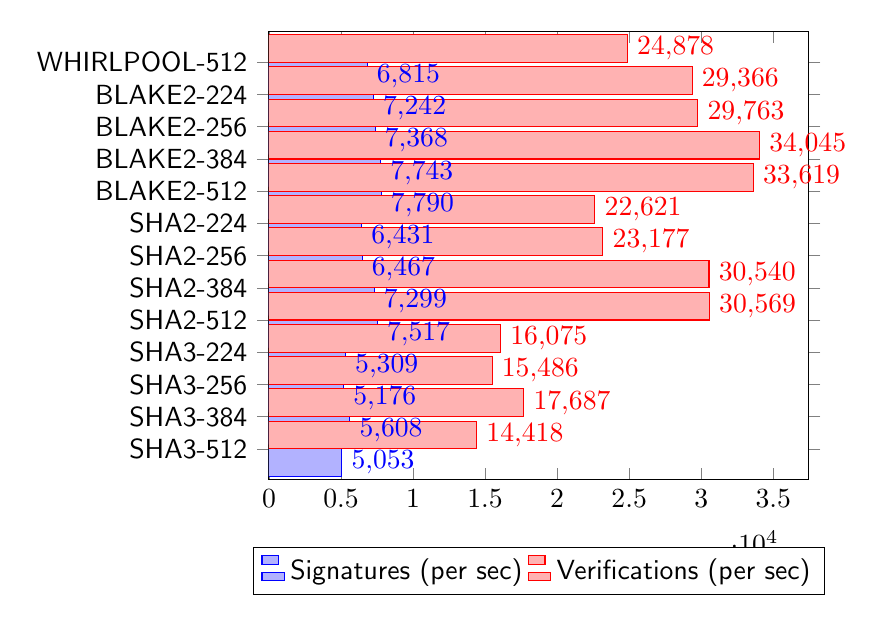
\begin{tikzpicture}
\begin{axis}[xbar=0pt, xmin=0, ytick=data, enlarge y limits=0.08, symbolic y coords={SHA3-512, SHA3-384, SHA3-256, SHA3-224, SHA2-512, SHA2-384, SHA2-256, SHA2-224, BLAKE2-512, BLAKE2-384, BLAKE2-256, BLAKE2-224, WHIRLPOOL-512}, y tick label style={/pgf/number format/1000 sep=}, nodes near coords, nodes near coords align={horizontal}, legend style={at={(0.5,-0.15)},anchor=north,legend columns=-1}]
\addplot
  coordinates
    {(5053,SHA3-512) (5608,SHA3-384) (5176,SHA3-256) (5309,SHA3-224)
     (7517,SHA2-512) (7299,SHA2-384) (6467,SHA2-256) (6431,SHA2-224)
     (7790,BLAKE2-512) (7743,BLAKE2-384) (7368,BLAKE2-256) (7242,BLAKE2-224)
     (6815,WHIRLPOOL-512)};

\addplot
  coordinates
    {(14418,SHA3-512) (17687,SHA3-384) (15486,SHA3-256) (16075,SHA3-224)
     (30569,SHA2-512) (30540,SHA2-384) (23177,SHA2-256) (22621,SHA2-224)
     (33619,BLAKE2-512) (34045,BLAKE2-384) (29763,BLAKE2-256) (29366,BLAKE2-224)
     (24878,WHIRLPOOL-512)};
\legend{Signatures (per sec), Verifications (per sec)}
\end{axis}
\end{tikzpicture}
\caption{BLISS-B-IV performance with various hash functions (Intel i7 6700 CPU @ 3.4GHz)}
\label{fig:bliss_b_hash_comparison}
\end{figure}

  \item BLAKE2-B lost out to Keccak in the SHA3 NIST competition, but it is an RFC (7693, draft).

\end{itemize}
\item A standalone performance analysis of the various hashing functions integrated into \textit{libsafecrypto} is provided in Figure \ref{fig:bliss_b_bytes_per_sec}:
\end{itemize}


\pgfplotsset{compat=1.13,width=14cm,height=22cm}
\begin{figure}[ht!]
\centering
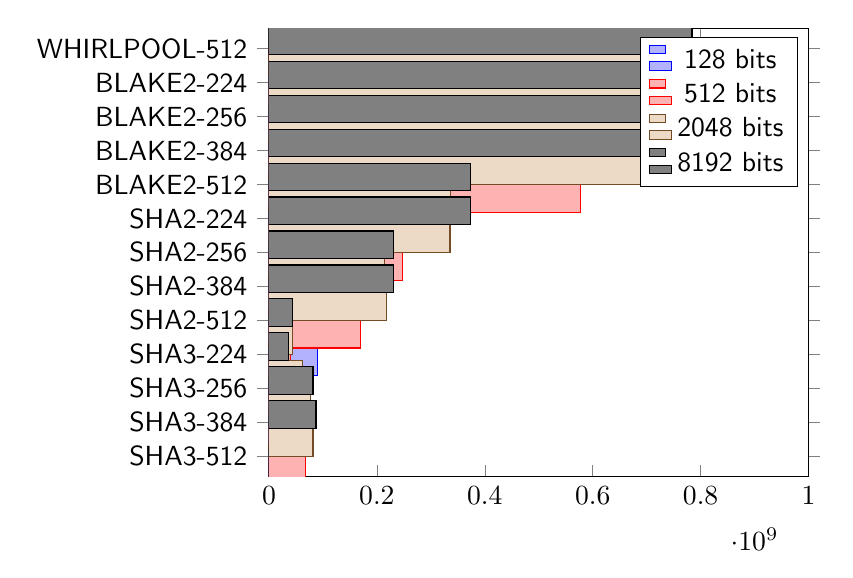
\begin{tikzpicture}
\begin{axis}[xbar=0pt, xmin=0, xmax=1000000000, ytick=data, enlarge y limits=0.05, symbolic y coords={SHA3-512, SHA3-384, SHA3-256, SHA3-224, SHA2-512, SHA2-384, SHA2-256, SHA2-224, BLAKE2-512, BLAKE2-384, BLAKE2-256, BLAKE2-224, WHIRLPOOL-512}, y tick label style={/pgf/number format/1000 sep=}]
\addplot
  coordinates
    {(41733600,SHA3-512) (66453490,SHA3-384) (33580860,SHA3-256) (26117498,SHA3-224) (90001193,SHA2-512) (111962015,SHA2-384) (137634227,SHA2-256) (133880238,SHA2-224) (318378956,BLAKE2-512) (245563664,BLAKE2-384) (143380969,BLAKE2-256) (341531003,BLAKE2-224) (63398434,WHIRLPOOL-512)};
\addplot
  coordinates
    {(67311617,SHA3-512) (47430787,SHA3-384) (60777654,SHA3-256) (39262358,SHA3-224) (169106491,SHA2-512) (176718677,SHA2-384) (246871771,SHA2-256) (250791574,SHA2-224) (577727014,BLAKE2-512) (582344548,BLAKE2-384) (589684613,BLAKE2-256) (591718794,BLAKE2-224) (131113251,WHIRLPOOL-512)};
\addplot
  coordinates
    {(81599679,SHA3-512) (76776751,SHA3-384) (62408720,SHA3-256) (43766790,SHA3-224) (217818471,SHA2-512) (214763352,SHA2-384) (335508930,SHA2-256) (336483310,SHA2-224) (718552357,BLAKE2-512) (729769587,BLAKE2-384) (738456684,BLAKE2-256) (732518714,BLAKE2-224) (149474568,WHIRLPOOL-512)};
\addplot
  coordinates
    {(87154415,SHA3-512) (81770554,SHA3-384) (36837864,SHA3-256) (44490799,SHA3-224) (231389170,SHA2-512) (230322287,SHA2-384) (372942248,SHA2-256) (373587750,SHA2-224) (771918396,BLAKE2-512) (748316921,BLAKE2-384) (788611685,BLAKE2-256) (783909562,BLAKE2-224) (158717452,WHIRLPOOL-512)};
\legend{128 bits, 512 bits, 2048 bits, 8192 bits}
\end{axis}
\end{tikzpicture}
\caption{Bytes per second performance of hash functions with varying message lengths [Intel i7 6700 CPU @ 3.4GHz]}
\label{fig:bliss_b_bytes_per_sec}
\end{figure}

\begin{itemize}
\item Profiling of the functional test executable for BLISS-B in \textit{valgrind/kcachegrind} shows that the performance bottlenecks are principally the hash function and the NTT, therefore small improvements to the associated functions provide reasonable performance gains.

\begin{itemize}

  \item Markku's Keccak/SHA3 has been optimised with some measures to manually perform loop unrolling so that the compiler doesn't have to use high (and potentially unstable) optimisation levels to achieve the same level of loop unrolling. However, this will be at the cost of an increased image size.

\begin{verbatim}
#ifdef SHA3_UNROLLED
    bc[0] = st[0] ^ st[0 + 5] ^ st[0 + 10] ^ st[0 + 15] ^ st[0 + 20];
    bc[1] = st[1] ^ st[1 + 5] ^ st[1 + 10] ^ st[1 + 15] ^ st[1 + 20];
    bc[2] = st[2] ^ st[2 + 5] ^ st[2 + 10] ^ st[2 + 15] ^ st[2 + 20];
    bc[3] = st[3] ^ st[3 + 5] ^ st[3 + 10] ^ st[3 + 15] ^ st[3 + 20];
    bc[4] = st[4] ^ st[4 + 5] ^ st[4 + 10] ^ st[4 + 15] ^ st[4 + 20];
#else
    for (i = 0; i < 5; i++) {
        bc[i] = st[i] ^ st[i + 5] ^ st[i + 10] ^ st[i + 15] ^ st[i + 20];
    }
#endif
\end{verbatim}

  \item Small indexing calculations in SHA-3 that are used repeatedly in loops where providing a large latency, therefore this has been replaced with 5 small LUTs to store the precomputed values.

\begin{verbatim}
    int i4mod5[5] = {4, 0, 1, 2, 3};
    int i1mod5[5] = {1, 2, 3, 4, 0};

    ...

    for (i = 0; i < 5; i++) {
        t = bc[i4mod5[i]] ^ ROTL64(bc[i1mod5[i]], 1);
        for (j = 0; j < 25; j += 5) {
            st[j + i] ^= t;
        }
    }
\end{verbatim}

As opposed to the original:

\begin{verbatim}
    for (i = 0; i < 5; i++) {
        t = bc[(i + 4) % 5] ^ ROTL64(bc[(i + 1) % 5], 1);
        for (j = 0; j < 25; j += 5) {
            st[j + i] ^= t;
        }
    }
\end{verbatim}
\end{itemize}
\end{itemize}


\clearpage
\subsubsection{Signature Restart}
\begin{itemize}
\item To improve the performance of the \textbf{Restart} if the rejection threshold is not met we have implemented a cheap but effective trick - every other time the signature algorithm is restarted the two random polynomials (sampled from a Gaussian distribution in the previous iteration) are simply swapped rather than re-generated, gaining approx. 10\%-25\% more signatures per second as shown in Figure \ref{fig:bliss_b_gaussian_swapping}.

\pgfplotsset{compat=1.13,width=15cm,height=7cm}
\begin{figure}[ht!]
\centering
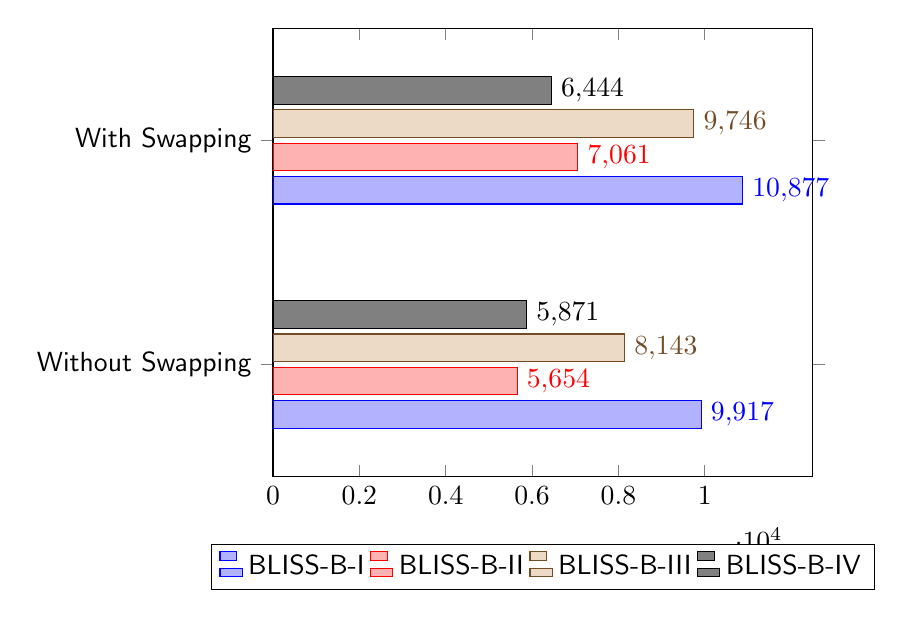
\begin{tikzpicture}
\begin{axis}[xbar, xmin=0, xmax=12500, xtick={0,2000,4000,6000,8000,10000}, ytick=data, enlarge y limits=0.5, symbolic y coords={Without Swapping, With Swapping}, y tick label style={/pgf/number format/1000 sep=}, nodes near coords, nodes near coords align={horizontal}, legend style={at={(0.5,-0.15)},anchor=north,legend columns=-1},]
\addplot coordinates {(9917,Without Swapping) (10877,With Swapping)};
\addplot coordinates {(5654,Without Swapping) (7061,With Swapping)};
\addplot coordinates {(8143,Without Swapping) (9746,With Swapping)};
\addplot coordinates {(5871,Without Swapping) (6444,With Swapping)};
\legend{BLISS-B-I, BLISS-B-II, BLISS-B-III, BLISS-B-IV}
\end{axis}
\end{tikzpicture}
\caption{Signatures per second performance of BLISS-B with no entropy coding and Restarts with/without Gaussian swapping [Intel i7 6700 CPU @ 3.4GHz]}
\label{fig:bliss_b_gaussian_swapping}
\end{figure}

\begin{itemize}
  \item In other schemes with a retrial a similar technique could be used. As BLISS must generate two Gaussian distributions it can quickly swap memory pointers rather than swapping the actual memory contents. Other schemes with only a single Gaussian distribution could employ methods to filter, scramble or partially update the existing distribution rather than create an entirely new polynomial using a Gaussian sampler.
\end{itemize}
\end{itemize}

\subsubsection{Entropy Coding}
\begin{itemize}
\item The signature is composed of three polynomials, $z_1$, $z_2$ and $c$. $z_1$ is a 12-bit code with a Gaussian distribution which can be exploited with an entropy coder to reduce the signature size. $z_2$ is a 2, 3 or 4 bit sparse polynomial (depending on the parameter set selected) that can also be readily compressed. The third polynomial $c$ contains random indices for an $n$ element polynomial and is short in length (12 to 39 elements) and therefore compression gains are minimal. The performance of BLISS-B signature compression is seen in Figure \ref{fig:bliss_b_signature_compression}, whilst the performance of the various entropy coders is shown in Figure \ref{fig:bliss_b_signature_compression_performance}.

\pgfplotsset{compat=1.13,width=14cm,height=8cm}
\begin{figure}[ht!]
\centering
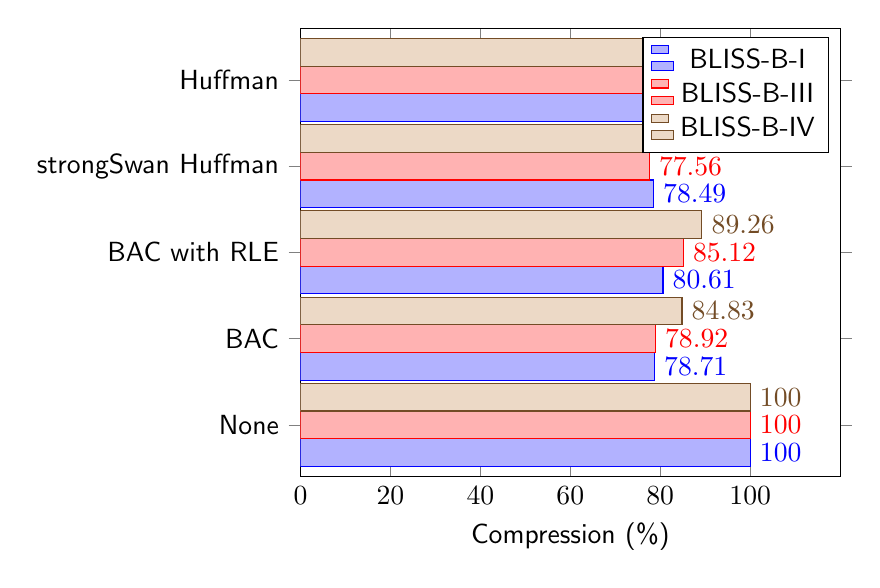
\begin{tikzpicture}
\begin{axis}[xbar=0pt, xlabel=Compression (\%), xmin=0, xmax=120, xtick={0,20,40,60,80,100}, ytick=data, enlarge y limits=0.15, symbolic y coords={None, BAC, BAC with RLE, strongSwan Huffman, Huffman}, y tick label style={/pgf/number format/1000 sep=}, nodes near coords, nodes near coords align={horizontal}]
\addplot coordinates {(100,None) (78.709,BAC) (80.606,BAC with RLE) (78.487,strongSwan Huffman) (80.721,Huffman)};
\addplot coordinates {(100,None) (78.918,BAC) (85.116,BAC with RLE) (77.555,strongSwan Huffman) (79.869,Huffman)};
\addplot coordinates {(100,None) (84.829,BAC) (89.264,BAC with RLE) (78.737,strongSwan Huffman) (80.36,Huffman)};
\legend{BLISS-B-I, BLISS-B-III, BLISS-B-IV}
\end{axis}
\end{tikzpicture}
\caption{BLISS-B Signature Compression with various entropy coders}
\label{fig:bliss_b_signature_compression}
\end{figure}

\pgfplotsset{compat=1.13,width=14cm,height=8cm}
\begin{figure}[ht!]
\centering
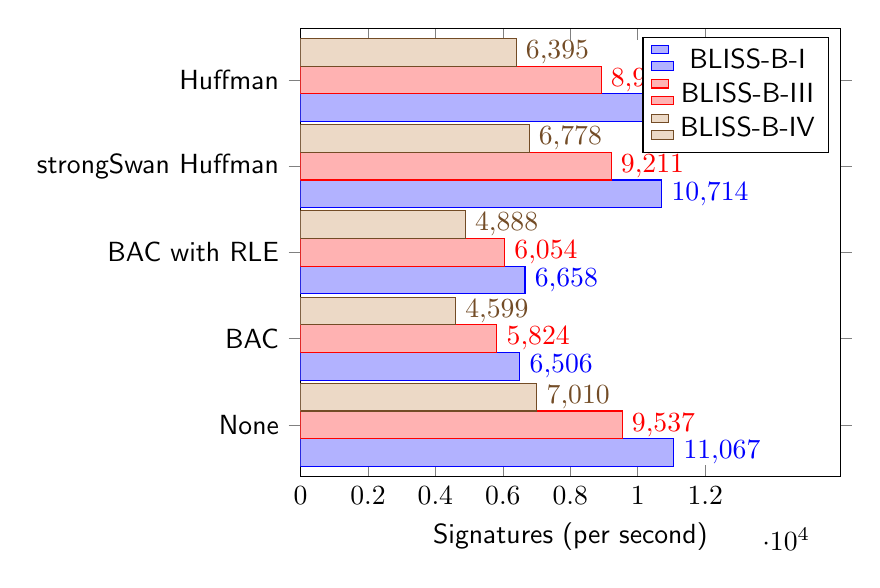
\begin{tikzpicture}
\begin{axis}[xbar=0pt, xlabel=Signatures (per second), xmin=0, xmax=16000, xtick={0,2000,4000,6000,8000,10000,12000}, ytick=data, enlarge y limits=0.15, symbolic y coords={None, BAC, BAC with RLE, strongSwan Huffman, Huffman}, y tick label style={/pgf/number format/1000 sep=}, nodes near coords, nodes near coords align={horizontal}]
\addplot coordinates {(11067,None) (6506,BAC) (6658,BAC with RLE) (10714,strongSwan Huffman) (10369,Huffman)};
\addplot coordinates {(9537,None) (5824,BAC) (6054,BAC with RLE) (9211,strongSwan Huffman) (8913,Huffman)};
\addplot coordinates {(7010,None) (4599,BAC) (4888,BAC with RLE) (6778,strongSwan Huffman) (6395,Huffman)};
\legend{BLISS-B-I, BLISS-B-III, BLISS-B-IV}
\end{axis}
\end{tikzpicture}
\caption{Performance of BLISS-B Signature Compression with various entropy coders [Intel i7 6700 CPU @ 3.4GHz]}
\label{fig:bliss_b_signature_compression_performance}
\end{figure}

\item The norms of the signature are currently checked by the signature algorithm, however this is not required and can be removed for a small performance gain.
\end{itemize}

\clearpage
\subsubsection{NTT/INTT}
\begin{itemize}

  \item The NTT loops have been modified to reduce some loop overhead in generating control variables, where possible they've been modified to encourage the compiler to use loop vectorisation and SIMD instructions.
  \item The NTT being used requires bit shuffling. This requires a function to swap each element of the polynomial with the element indexed by the bit reverse of it's index (\textit{see inverse\_shuffle\_32() in ntt.c}). For example, ARM instruction sets have a bit reverse instruction that can readily obtain the correct index for the swap operation.

\begin{verbatim}

UINT32 sc_bit_reverse_32(UINT32 x)
{
#ifdef __arm__
    UINT32 y;
    __asm__("rbit %0, %1\n" : "=r"(y) : "r"(x));
    return y;
#else
    x = (((x & 0xaaaaaaaa) >> 1) | ((x & 0x55555555) << 1)); // Swap odd and even
    x = (((x & 0xcccccccc) >> 2) | ((x & 0x33333333) << 2)); // Swap pairs
    x = (((x & 0xf0f0f0f0) >> 4) | ((x & 0x0f0f0f0f) << 4)); // Swap nibbles
    x = (((x & 0xff00ff00) >> 8) | ((x & 0x00ff00ff) << 8)); // Swap bytes
    return (x >> 16) | (x << 16);                            // Swap pairs of bytes
#endif
}

...

// Make use of a bit reversal instruction
UINT32 bits = 32 - sc_ctz_32(n);
for (i = 1; i < n-1; i++) {       // 00..0 and 11..1 remain same
    UINT32 r = sc_bit_reverse_32(i);
    r >>= bits;
    if (i < r) {
        SINT32 x = v[i];
        v[i] = v[r];
        v[r] = x;
    }
}
\end{verbatim}

  \item On x86 we can use the gcc \textit{builtin\_ctz} function (if available) to provide a more optimal bit reversal function by incrementing the MSB's to obtain bit reversal.

\begin{verbatim}
// If a BUILTIN funtion exists for CTZ then inverse incremental
// counting can be achieved by incrementing the MSB's
UINT32 bits = sc_ctz_32(n) - 1;
j = n >> 1;
for (i = 1; i < n - 1;) {       // 00..0 and 11..1 remain same
    if (i < j) {
        SINT32 x = v[i];
        v[i] = v[j];
        v[j] = x;
    }
    UINT32 mask = i++;
    mask ^= i;
    UINT32 len = sc_ctz_32(i);
    mask <<= bits - len;
    j ^= mask;
}
\end{verbatim}

  \item A fallback method is provided that increments the MSB's without the help of the \textit{builtin\_ctz} function and provides a generic solution. However, this method requires a \textit{while} loop.

\begin{verbatim}
// This is the fallback method that also increments the MSB's
j = n >> 1;
for (i = 1; i < n - 1; i++) {       // 00..0 and 11..1 remain same
    if (i < j) {
        SINT32 x = v[i];
        v[i] = v[j];
        v[j] = x;
    }
    k = n;
    do {
        k >>= 1;
        j ^= k;
    } while ((j & k) == 0);
}
\end{verbatim}

  \item As the performance of the loops in the NTT are critical it was seen that reduction scheme specific implementations of the main NTT function were beneficial to performance. So rather than set a function pointer to use the desired multiplication and modular reduction routine, specific NTT functions were added for each reduction scheme that remove the overhead of function calls and in addition permit the compiler to perform loop unrolling and loop vectorisation, leading to some reasonable performance gains. A summary describing the performance gains achieved through simple optimisation of the NTT is shown in Figure \ref{fig:bliss_b_optimised_ntt}.

\pgfplotsset{compat=1.13,width=11cm,height=9cm}
\begin{figure}[ht!]
\centering
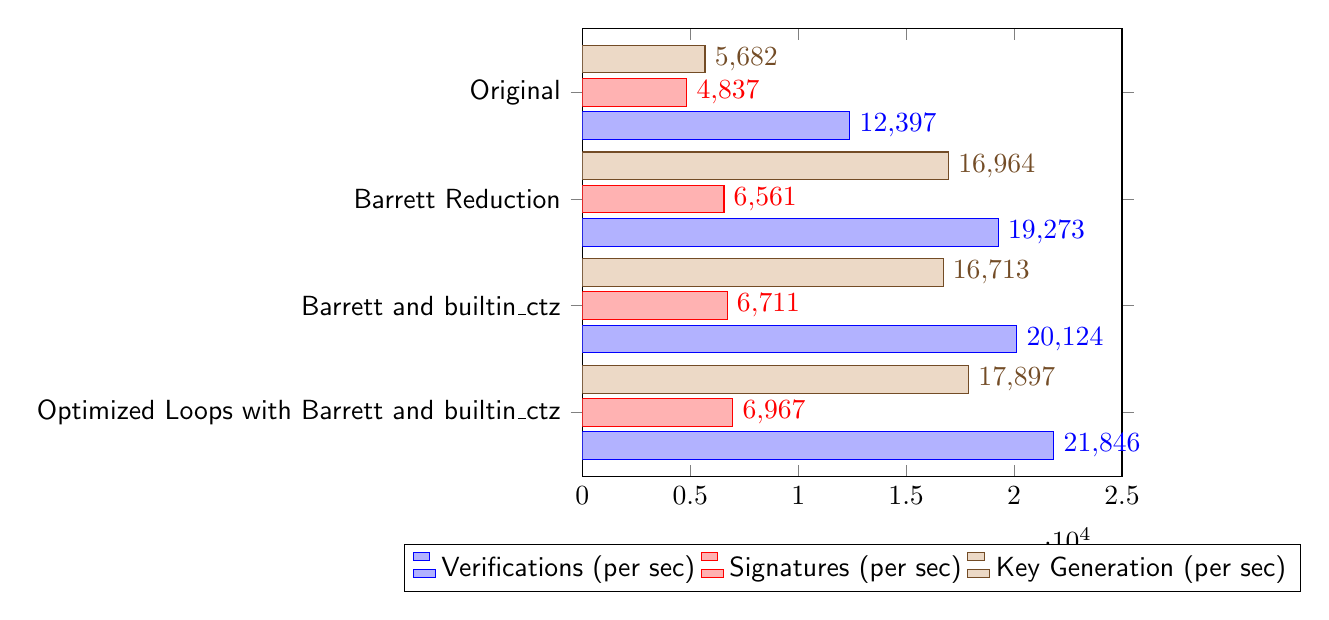
\begin{tikzpicture}
\begin{axis}[xbar, xmin=0, xmax=25000, xtick={0,5000,10000,15000,20000,25000}, ytick=data, symbolic y coords={Optimized Loops with Barrett and builtin\_ctz, Barrett and builtin\_ctz, Barrett Reduction, Original}, enlarge y limits=0.2, y tick label style={/pgf/number format/1000 sep=}, nodes near coords, nodes near coords align={horizontal}, legend style={at={(0.5,-0.15)},anchor=north,legend columns=-1},]
\addplot coordinates {(21846,Optimized Loops with Barrett and builtin\_ctz) (20124,Barrett and builtin\_ctz) (19273,Barrett Reduction) (12397,Original)};
\addplot coordinates {(6967,Optimized Loops with Barrett and builtin\_ctz) (6711,Barrett and builtin\_ctz) (6561,Barrett Reduction) (4837,Original)};
\addplot coordinates {(17897,Optimized Loops with Barrett and builtin\_ctz) (16713,Barrett and builtin\_ctz) (16964,Barrett Reduction) (5682,Original)};
\legend{Verifications (per sec), Signatures (per sec), Key Generation (per sec)}
\end{axis}
\end{tikzpicture}
\caption{Performance gains from optimised NTT loops [Intel i7 6700 CPU @ 3.4GHz]}
\label{fig:bliss_b_optimised_ntt}
\end{figure}

  \item The NTT roots of unity tables are stored using the minimum bit width type required. When these coefficients are used in multiplication routines they are typically cast to an int64\_t or a double, and within the loop operations of the NTT/INTT they are read infrequently relative to other variables. Therefore using the minimal storage type reduces the memory use within the image whilst having no impact on performance.
\end{itemize}

\subsubsection{CSPRNG}
\begin{itemize}

  \item A range of PRNG's are provided by the SAFEcrypto library: ISAAC \cite{issac}, KISS \cite{kiss}, AES-PRNG (utilizes Brian Gladman's AES \cite{aes_gladman}) and CHACHA20-CSPRNG \cite{chacha20_csprng}.
  \item A functional test of the various CSPRNG options was used to determine their relative performance - the results are shown in Figure \ref{fig:hash_mbyte_per_sec}.

\pgfplotsset{compat=1.13,width=10cm,height=9cm}
\begin{figure}[ht!]
\centering
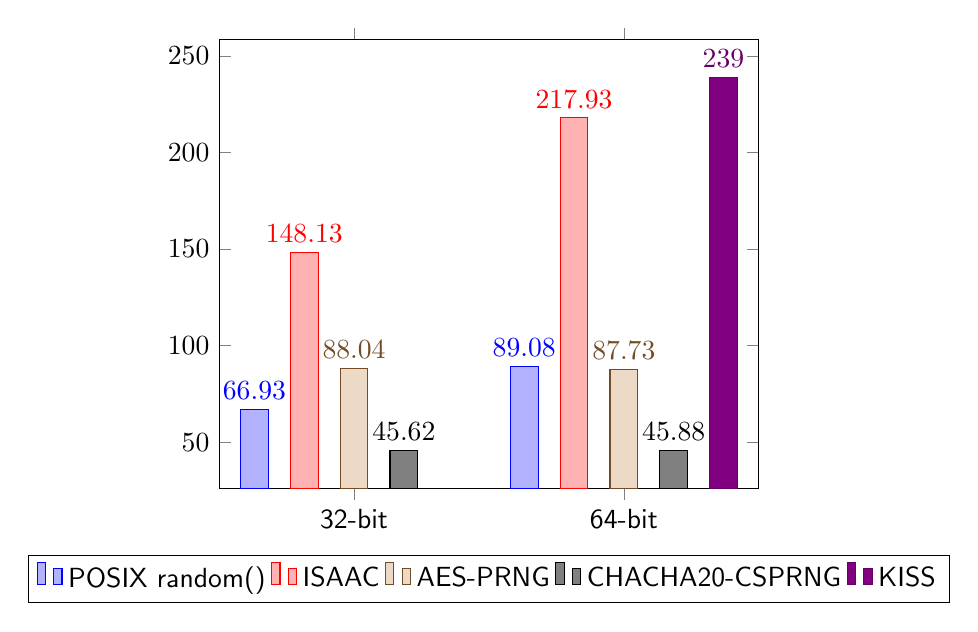
\begin{tikzpicture}
\begin{axis}[ybar=8pt, xtick=data, enlarge x limits=0.5, symbolic x coords={32-bit, 64-bit}, x tick label style={/pgf/number format/1000 sep=}, nodes near coords, nodes near coords align={vertical}, legend style={at={(.5,-0.15)},anchor=north,legend columns=-1}]
\addplot coordinates {(32-bit, 66.933) (64-bit, 89.083)};
\addplot coordinates {(32-bit, 148.129) (64-bit, 217.928)};
\addplot coordinates {(32-bit, 88.041) (64-bit, 87.73)};
\addplot coordinates {(32-bit, 45.615) (64-bit, 45.882)};
\addplot coordinates {(64-bit, 239.004)};
\legend{POSIX random(), ISAAC, AES-PRNG, CHACHA20-CSPRNG, KISS}
\end{axis}
\end{tikzpicture}
\caption{Performance of various CSPRNG schemes in MByte/sec [Intel i7 6700 CPU @ 3.4GHz]}
\label{fig:hash_mbyte_per_sec}
\end{figure}

\noindent \textbf{NOTE: KISS is 64-bit only, we probably need to implement the 32-bit version for comparison purposes.}

\item The performance of BLISS-B with no entropy coding whilst using a range of CSPRNG's is shown in Figure \ref{fig:bliss_b_csprng_comparison}. As expected there is no real difference in improvement for the verification operation as it requires no random number generation. The higher performance of KISS and ISAAC translates to higher performance within BLISS-B, with both CSPRNG's offering very similar performance.

\pgfplotsset{compat=1.13,width=15cm,height=10cm}
\begin{figure}[ht!]
\centering
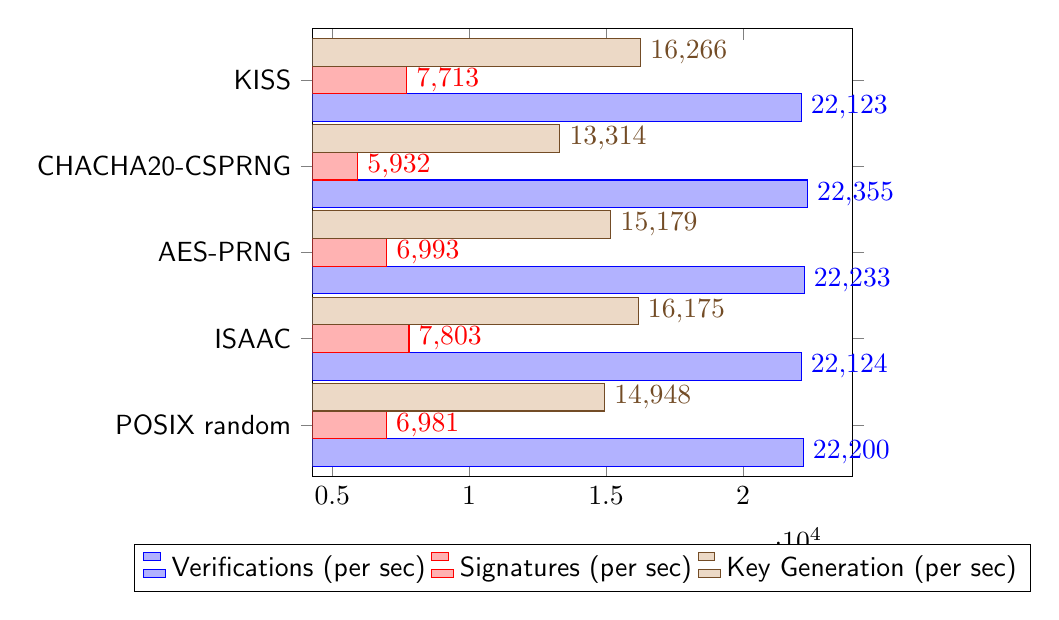
\begin{tikzpicture}
\begin{axis}[xbar=0pt, ytick=data, enlarge y limits=0.15, symbolic y coords={POSIX random, ISAAC, AES-PRNG, CHACHA20-CSPRNG, KISS}, y tick label style={/pgf/number format/1000 sep=}, nodes near coords, nodes near coords align={horizontal}, legend style={at={(.5,-0.15)},anchor=north,legend columns=-1}]
\addplot coordinates {(22200,POSIX random) (22124,ISAAC) (22233,AES-PRNG) (22355,CHACHA20-CSPRNG) (22123,KISS)};
\addplot coordinates {(6981,POSIX random) (7803,ISAAC) (6993,AES-PRNG) (5932,CHACHA20-CSPRNG) (7713,KISS)};
\addplot coordinates {(14948,POSIX random) (16175,ISAAC) (15179,AES-PRNG) (13314,CHACHA20-CSPRNG) (16266,KISS)};
\legend{Verifications (per sec), Signatures (per sec), Key Generation (per sec)}
\end{axis}
\end{tikzpicture}
\caption{Performance of various CSPRNG schemes in BLISS-B-IV [Intel i7 6700 CPU @ 3.4GHz]}
\label{fig:bliss_b_csprng_comparison}
\end{figure}

\end{itemize}


\clearpage
\subsection{Verification}

\begin{itemize}
\item Reject if $||(z_1 | 2^d . z_2)||_2 > B_2$
\item Reject if $||(z_1 | 2^d . z_2)||_\infty > B_2$
\item Accept if $c = H(\lfloor a_1 . z_1 + q . c \rceil_d + z_2 mod p, \mu)$
\end{itemize}

Verification utilises some of the same functions as signing (NTT, Hashing, checking the signature norms) so achieves the same gains when these are improved.

\begin{itemize}
\item There are some operations that require a polynomial to be reduced using \textit{2q} or \textit{p} rather than \textit{q}. These have also been accelerated using Barrett and Floating Point reduction techniques, taking care to structure the code such that automatic vectorisation is enabled by the compiler.
\end{itemize}



\subsection{General Performance Improvements}

\begin{itemize}
\item Intermediate storage is achieved using heap memory allocated when the schemes call the \textit{create()} functions. This memory is released when the scheme is destroyed. This means that when any cryptographic functions are called there is no dynamic memory allocation or static memory used to store intermediate variables.
\item Integer and floating point types of 32-bit or larger are preferred on x86/AMD64 as the compiler can exploit SIMD/AVX auto-vectorization. This compiler optimization is to be investigated further for other microprocessor architectures.
\end{itemize}


\subsection{Summary}

The original hilabliss/BLZZRD implementations of BLISS are reference designs used to show the algorithms and functional operation of the signature scheme; as such they are intended to be non-optimal.

We have shown that the use of a Binary Arithmetic Coder within BLZZRD is sub-optimal in terms of performance, both as a Gaussian Sampler and an entropy coder. Huffman is significantly faster, whilct as a Gaussian Sampler it is statistically poor.

Also, hilabliss/BLZZRD and many other lattice-based cryptographic schemes are using SHA-3 as a hash function when implementing a random oracle. It is shown that this is a poor choice in terms of performance if not security. Therefore it is strongly suggested that a more optimal choice of hash would be SHA-2 or BLAKE2-B, both are standardized and strong hash functions in line with SHA-3.

The performance gains that have been achieved are summarised in Figures \ref{fig:bliss_b_no_entropy_comparison} and \ref{fig:bliss_b_entropy_comparison}. In this diagram the original algorithm is shown in comparison to (a) a version in which the NTT's and modular reduction have been optimised and (b) a version in which the the BLISS-B algorithm has been fully optimised with the addition of the ISAAC as a CSPRNG and BLAKE2 as a hash function. In all of these implementations entropy coding is disabled.

\noindent \textbf{I hope to add a multithreaded version in which the CSPRNG and Gaussian Sampler have been placed into worker threads which should be significantly faster again, even if it is cheating!}

\pgfplotsset{compat=1.13,width=12cm,height=8cm}
\begin{figure}[ht!]
\centering
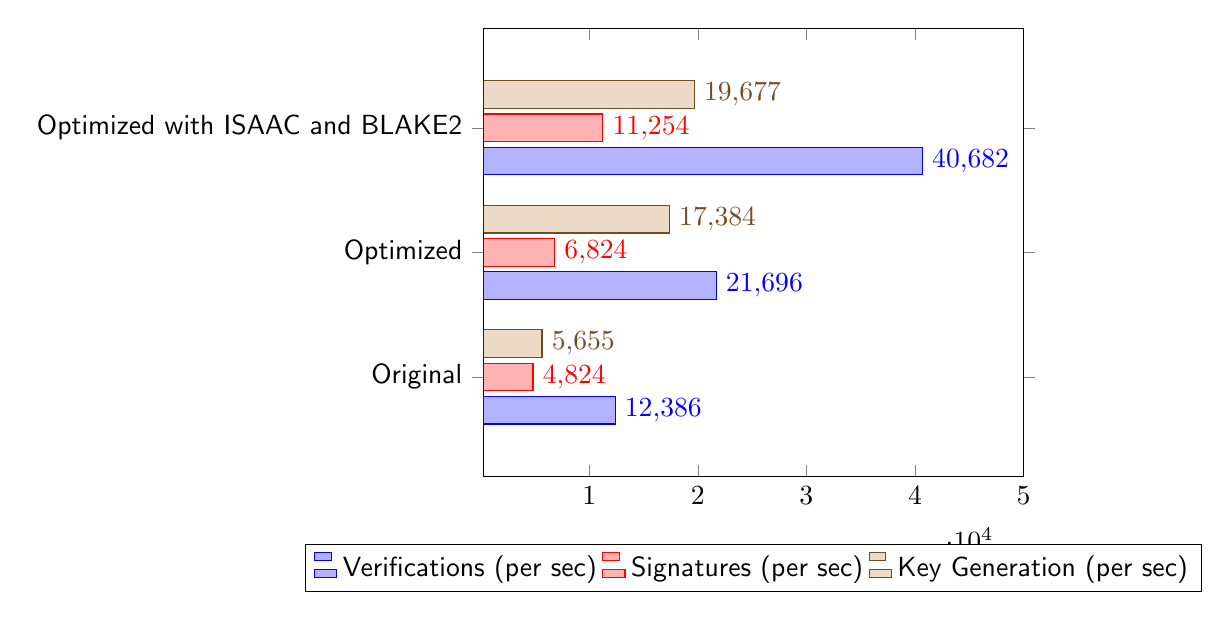
\begin{tikzpicture}
\begin{axis}[xbar=2pt, xmax=50000, ytick=data, enlarge y limits=0.4, symbolic y coords={Original, Optimized, Optimized with ISAAC and BLAKE2}, y tick label style={/pgf/number format/1000 sep=}, nodes near coords, nodes near coords align={horizontal}, legend style={at={(.5,-0.15)},anchor=north,legend columns=-1}]
\addplot coordinates {(40682,Optimized with ISAAC and BLAKE2) (21696,Optimized) (12386,Original)};
\addplot coordinates {(11254,Optimized with ISAAC and BLAKE2) (6824,Optimized) (4824,Original)};
\addplot coordinates {(19677,Optimized with ISAAC and BLAKE2) (17384,Optimized) (5655,Original)};
\legend{Verifications (per sec), Signatures (per sec), Key Generation (per sec)}
\end{axis}
\end{tikzpicture}
\caption{Performance of SAFEcrypto BLISS-B-IV with no entropy coding [Intel i7 6700 CPU @ 3.4GHz]}
\label{fig:bliss_b_no_entropy_comparison}
\end{figure}

\pgfplotsset{compat=1.13,width=12cm,height=8cm}
\begin{figure}[ht!]
\centering
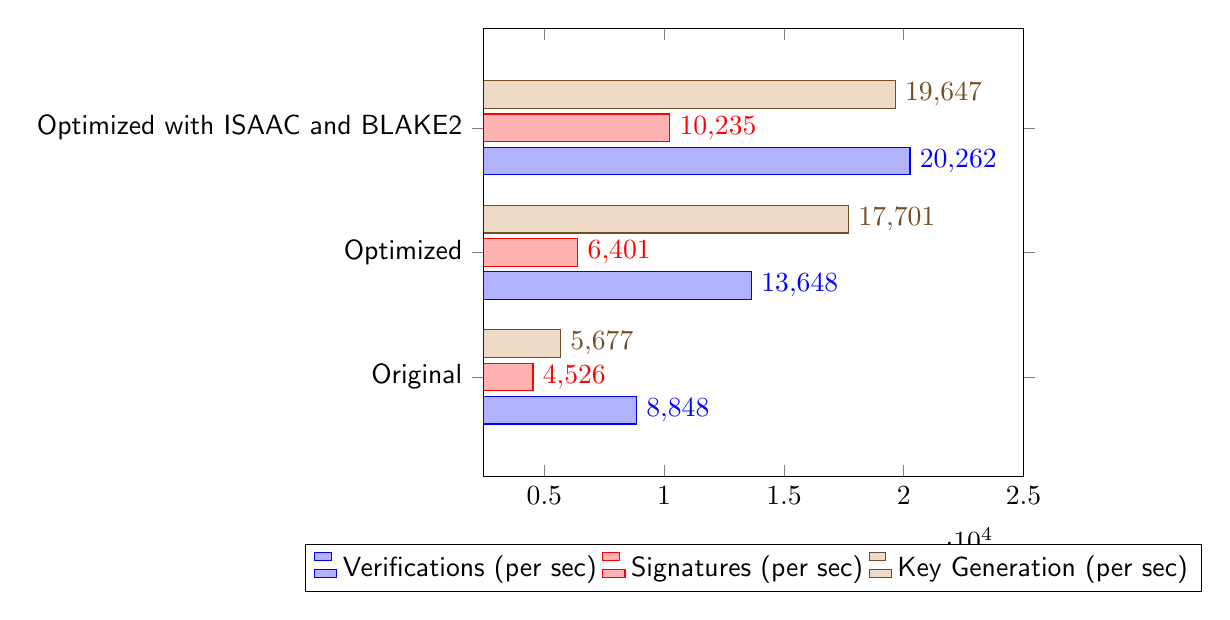
\begin{tikzpicture}
\begin{axis}[xbar=2pt, xmax=25000, ytick=data, enlarge y limits=0.4, symbolic y coords={Original, Optimized, Optimized with ISAAC and BLAKE2}, y tick label style={/pgf/number format/1000 sep=}, nodes near coords, nodes near coords align={horizontal}, legend style={at={(.5,-0.15)},anchor=north,legend columns=-1}]
\addplot coordinates {(20262,Optimized with ISAAC and BLAKE2) (13648,Optimized) (8848,Original)};
\addplot coordinates {(10235,Optimized with ISAAC and BLAKE2) (6401,Optimized) (4526,Original)};
\addplot coordinates {(19647,Optimized with ISAAC and BLAKE2) (17701,Optimized) (5677,Original)};
\legend{Verifications (per sec), Signatures (per sec), Key Generation (per sec)}
\end{axis}
\end{tikzpicture}

\textbf{[Put comparisons to other implementations of BLISS-B in here as it is compatible.]}
\caption{Performance of SAFEcrypto BLISS-B-IV with Huffman compression [Intel i7 6700 CPU @ 3.4GHz]}
\label{fig:bliss_b_entropy_comparison}
\end{figure}


\clearpage
In Figure \ref{fig:bliss_b_comparison} the original implementation of BLZZRD \cite{markku_blzzrd} is compared to a compatible implementation created using the SAFEcrypto library (i.e. SHA-3, Binary Arithmetic Coding and Blinding countermeasures). Verification is shown to be approximately 14\% slower using the SAFEcrypto library which can be attributed to the poor performance of the BAC decoder (\textit{some more effort could be exercised in trying to improve this}). However, the signature performance is approximately 25\% faster whilst key generation is significantly faster by 330\%.

A higher performance version of BLZZRD, here called \textit{BLZZRD+}, has been implemented to address the poor performance associated with the BAC and hash. BLZZRD+ utilises the more efficient BLAKE2 hash function, Ziggurat Gaussian Sampling and Huffman coding, whilst maintaining blinding countermeasures. As such it gains much greater performance for signing and verifying, being approximately 250\% and 170\% faster respectively than the original BLZZRD implementation.

\textit{The paper in \cite{markku_blzzrd} quotes performance on a 2.5GHz i7 in milliseconds per operation. To scale these figures for use here they have been inverted to convert to operations per second and muliplied by $1.36$ to scale to a 3.4GHz i7.}

\pgfplotsset{compat=1.13,width=12cm,height=8cm}
\begin{figure}[ht!]
\centering
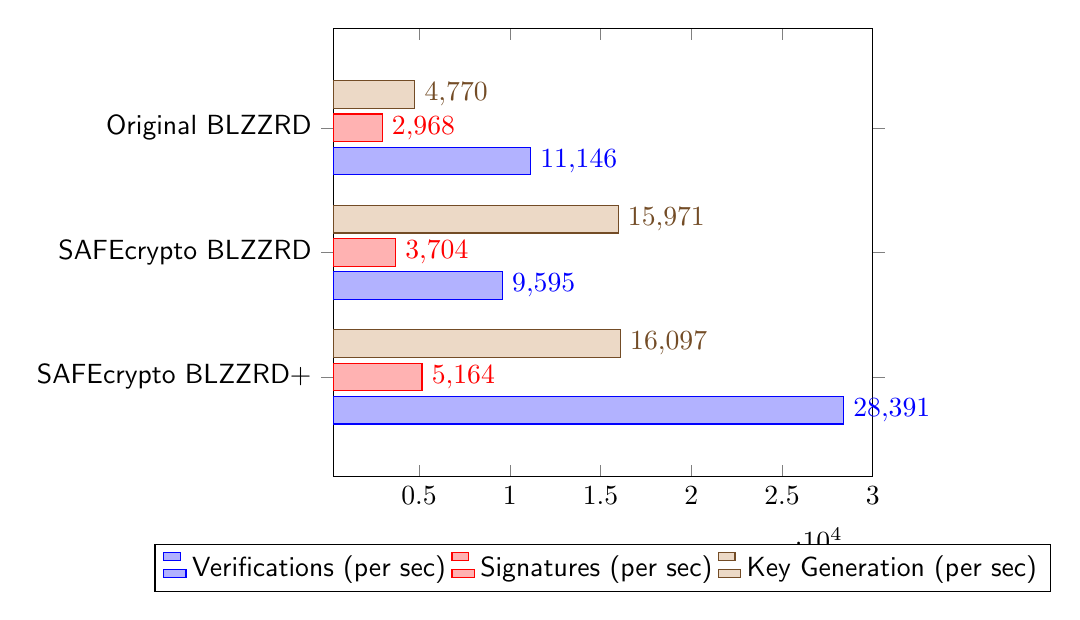
\begin{tikzpicture}
\begin{axis}[xbar=2pt, xmax=30000, ytick=data, enlarge y limits=0.4, symbolic y coords={SAFEcrypto BLZZRD+, SAFEcrypto BLZZRD, Original BLZZRD}, y tick label style={/pgf/number format/1000 sep=}, nodes near coords, nodes near coords align={horizontal}, legend style={at={(.5,-0.15)},anchor=north,legend columns=-1}]
\addplot coordinates {(28391,SAFEcrypto BLZZRD+) (9595,SAFEcrypto BLZZRD) (11146,Original BLZZRD)};
\addplot coordinates {(5164,SAFEcrypto BLZZRD+) (3704,SAFEcrypto BLZZRD) (2968,Original BLZZRD)};
\addplot coordinates {(16097,SAFEcrypto BLZZRD+) (15971,SAFEcrypto BLZZRD) (4770,Original BLZZRD)};
\legend{Verifications (per sec), Signatures (per sec), Key Generation (per sec)}
\end{axis}
\end{tikzpicture}
\caption{Performance comparison of SAFEcrypto BLZZRD-IV [Intel i7 6700 CPU @ 3.4GHz]}
\label{fig:bliss_b_comparison}
\end{figure}


%\section{IBE and AKE}

This section aims to describe the IBE and AKE schemes developed as part of the SAFEcrypto project from an implementation perspective. It should be noted that both schemes are almost identical.

\subsection{Key Generation}

IBE and AKE rely upon the algorithm in Figure \ref{fig:ibe_keygen} to generate the public key \textit{h} and \textit{Master Secret Key \textbf{B}}. In IBE the \textit{Extract} function (see Figure \ref{fig:ibe_extract}) is detached from Key Generation as it is required to derive a secret key for each user from the master key, whilst it is incorporated into AKE's key generation function as it effectively has only one user \textit{id} (see Figure \ref{fig:ake_digital_signature}).

The key generation function is quite involved. The principle operations involve repeated trials of the randomly generated keys \textit{(f, g)} with Extended GCD and GCD functions until co-prime relationships have been found. An added complexity of this step is the need to compute the GCD's using large integer arithmetic in order to obtain an integer GCD and Bezout coefficients.

\begin{figure}[H]
\centering
\includegraphics[width=11cm]{ibe_keygen.png}
\caption{IBE KeyGen}
\label{fig:ibe_keygen}
\end{figure}

\begin{figure}[H]
\centering
\includegraphics[width=11cm]{ibe_extract.png}
\caption{IBE Extract}
\label{fig:ibe_extract}
\end{figure}

\begin{figure}[H]
\centering
\includegraphics[width=9cm]{ake_hash_and_sign.png}
\caption{Whole is less... Digital Signature Scheme}
\label{fig:ake_digital_signature}
\end{figure}

\subsection{IBE Encrypt and Decrypt}

The IBE encrypt and decrypt operations involve mapping binary bits onto the lattice and recovering them - in a similar manner to the RLWE encryption scheme. It should be noted that this scheme uses large modulus values to reduce the failure probability of the encryption operation - therefore decryption failures should be expected at a negligible rate during any testing of the scheme.

\begin{figure}[H]
\centering
\includegraphics[width=14cm]{ibe_encrypt.png}
\caption{IBE Encrypt}
\label{fig:ibe_encrypt}
\end{figure}

\begin{figure}[H]
\centering
\includegraphics[width=14cm]{ibe_decrypt.png}
\caption{IBE Decrypt}
\label{fig:ibe_decrypt}
\end{figure}

\subsection{Extract and Signing}

AKE signing is almost identical to IBE extract, both requiring Gaussian Sampling over a lattice.

\subsection{AKE Signatures with Message Recovery}

AKE also defines a \textit{Signature with Message Recovery} scheme (see Figure \ref {fig:ake_signature_with_recovery}) that can be used to produce smaller signatures at the cost of more CPU cycles. Instead of sending the signature as $(s_1, m)$ and recovering $s_2$, it is instead transmitted as $(s_1, s_2)$ and the message $m$ is recovered by the verifier.

\begin{figure}[H]
\centering
\includegraphics[width=11cm]{ake_with_message_recovery.png}
\caption{Whole is less... Digital Signature Scheme with Message Recovery}
\label{fig:ake_signature_with_recovery}
\end{figure}


\subsection{Software Implementation}

The generic AKE scheme shown in Figure \ref{fig:generic_ake} indicates that the signature keys are typically generated once whilst the KEM keys are generated on a per-session basis. Therefore the complexity of AKE \textit{SigKeyGen} should not be a burden as it can effectively be treated as an off-line computation. Real performance gains in a system will be achieved by optimising the regularly used \textit{Sign, Verify, KEMKeyGen, Encapsulate} and \textit{Decapsulate} operations. Similarly for IBE, the regularly used \textit{Extract, Encrypt} and \textit{Decrypt} functions should be the focus of optimisation.

\begin{figure}[H]
\centering
\includegraphics[width=9cm]{ake_kem.png}
\caption{AKE KEM}
\label{fig:ake_kem}
\end{figure}

\begin{figure}[H]
\centering
\includegraphics[width=7cm]{generic_ake.png}
\caption{A Generic AKE Construction from a KEM and a Digital Signature}
\label{fig:generic_ake}
\end{figure}

The main areas of work that are foreseen in implementing both IBE and AKE within the SAFEcrypto library are the following:

\begin{enumerate}[1]
\item A generic implementation of the IBE \textit{Master\_Keygen} function to be used by both IBE and AKE.
\begin{enumerate}[a]
\item Big integer arithmetic functions (add/sub, multiply, divide, GCD) [currently using GMP, libtommath has been added to the build system].
\item XGCD with integer polynomial coefficients (NTL and FLINT have this function and can be used as a reference).
\end{enumerate}
\item Implementing a discrete Gaussian Sampling scheme over a lattice using the polynomial basis \textit{\textbf{B}}, i.e. IBE Extract and AKE SigKeyGen.
\item Verifying the correctness of the already implemented AKE KEM as one of the parameter sets appears to be incorrect.
\item Acceleration of the Whole KEM scheme, in particular inversion modulo 2 used in \textit{KEMKeyGen}.
\item Re-factoring the RLWE Encryption encrypt/decrypt source code for IBE encrypt/decrypt.
\end{enumerate}

%\chapter{Proposals}
\label{ch_proposals}

\section{API}

A C API is preferred as it is highly portable and permits rapid integration with other programming languages and applications.


\subsection{Creation}

\begin{itemize}
\item The library will use a structure to store all of the parameters related to a single instance of SAFEcrypto.

\begin{verbatim}
      extern safecrypto *safecrypto_create(const char *algorithm);
\end{verbatim}

\item This structure must be created for a particular algorithm using a human readable string identifier.
\item If the structure cannot be created a NULL pointer is returned which the user must check for.
\item A destruct function is used to free all resources allocated to the SAFEcrypto structure and all internal memory resources.
\end{itemize}

\begin{verbatim}
    extern int32_t safecrypto_destroy(safecrypto *sc);
\end{verbatim}


\subsection{Debug Printing}

\begin{itemize}
\item Macros should be provided to allow users to insert arbitrary print statements that will be removed during compilation of a released library.
\item Debug macros should be multi-level to provide a hierarchy of debug statements to improve the efficiency of bug finding.
\item The debug logging facility should be thread-safe to allow its use in those algorithms which make use of concurrency.
\item The debug logging facility should print to a user specified file with a default name.
\item Variadic print functions will be used that provide indentical functional to \textit{printf~()}:
\end{itemize}

\vspace{1em}
\textit{Example use:}

\indent\begin{verbatim}
    int *p = NULL;
    …

    if (p == NULL) {
        SC_LOG_ERROR(sc, SC_NULL_PTR);
        return SC_FUNC_FAILURE;
    }
\end{verbatim}


\subsection{Error Queue}

\begin{itemize}
\item An error queue facility similar to that used by OpenSSL will be used:

\begin{verbatim}
    extern uint32_t safecrypto_err_get_error(safecrypto *sc);
    extern uint32_t safecrypto_err_peek_error(safecrypto *sc);
    extern uint32_t safecrypto_err_get_error_line(safecrypto *sc,
        const char **file, int32_t *line);
    extern uint32_t safecrypto_err_peek_error_line(safecrypto *sc,
        const char **file, int32_t *line);
    extern void safecrypto_err_clear_error(safecrypto *sc);
\end{verbatim}

\item An error message including an error code, file name and line number will be buffered in a finite length queue of errors.
\item If the queue is full new errors will be discarded such that the possible root cause of an issue will remain in the buffer.
\item Error messages will automatically utilise the debug printing facility if it is enabled.
\item It is the user’s responsibility to manage the error queue.
\end{itemize}

\subsection{Parameters}

\begin{itemize}
\item Store all parameters as arrays of length 1 or greater using dynamic memory.
\item All parameters will have a unique human readable name used for identification.
\item All parameters are stored in some form of linked list with nodes composed of struct’s containing all necessary details (name, type, length and a void* pointer to the array of data).

\begin{verbatim}
    typedef enum sc_param_type {
        SC_PARAM_UINT8 = 0,
        SC_PARAM_UINT16,
        SC_PARAM_UINT32,
        SC_PARAM_INT8,
        SC_PARAM_INT16,
        SC_PARAM_INT32,
        SC_PARAM_FLOAT,
        SC_PARAM_DOUBLE,
    } sc_param_type_e;

    typedef struct sc_param {
        char name[SC_MAX_NAME_LEN];
        safecrypto_param_type_e type;
        void *value;
        int32_t length;
    } sc_param_t;
\end{verbatim}


\item A simple API function is provided to obtain a pointer to the struct containing the parameter with a specified name:

\begin{verbatim}
    extern safecrypto_param_t *safecrypto_param_get(safecrypto *sc,
        const char *name);
\end{verbatim}

\item Where the name of parameters is unknown, functions are provided to iteratively parse the linked list:

\begin{verbatim}
    extern safecrypto_param_t *safecrypto_param_get_first(safecrypto *sc);
    extern safecrypto_param_t *safecrypto_param_get_next(safecrypto *sc,
        safecrypto_param_t *param);
\end{verbatim}

\item When each allgorithm is initialised it MUST populate the linked list of parameters with an initial set of known good parameters.
\item A helper function is provided to allow parameters for the selected algorithm to be configured according to the minimum number of permitted security bits.
\end{itemize}

\vspace{1em}
\textit{Example usage:}

\indent\begin{verbatim}
    safecrypto *sc = safecrypto_create(“Algorithm A”);
    …

    // List all parameters
    safecrypto_param_t *param = safecrypto_param_get_first(sc);
    while (param != NULL ) {
        // Print the parameter details
        printf(“Parameter %s has %d elements:\n”, param->name, param->length);
        switch (param->type)
        {
        case SC_PARAM_UINT8:
            uint8_t *p = (uint8_t *)param->value;
            for (int i=0; i<param->length; i++)
                printf(“%02X ”, (int)(*p++));
            printf(“\n”);
            break;
        case SC_PARAM_UINT16:
        ...
        default:;
        }
        param = safecrypto_param_get_next(sc, param);
    }
\end{verbatim}



\newpage
\section{Dynamic Configuration}

\subsection{Assumptions}

\begin{itemize}
\item The API provides a method that permits arbitrary parameters to be created, modified and used by any algorithm.
\end{itemize}

\subsection{Goals}

\begin{itemize}
\item As algorithms are developed the necessary mathematical and cryptographic functions will be implemented into a library of functions known as the toolbox.
\item The functions within the toolbox will be configurable at compile time to support optimizations for various processor architectures.
\item The toolbox will provide the functionality required to implement more abstract functions, thereby reducing development time and providing a similar platform on which to compare algorithms.
\end{itemize}

\subsection{Proposed Implementation}

\begin{itemize}
\item All functions/classes within the toolbox will be named with the prefix tb to enable their easy identification.
\item An additional prefix will be used to idenify the type of function (e.g.\ prf for pseudo random function, arith for arithmetic functions such as polynomial or matrix manipulation, thread for concurrency functions, etc.)
\item These functions MUST be used where any significant data processing occurs.
\item If functionality offered by the toolbox is not available then it must be implemented within the toolbox if it is believed it can be re-used elsewhere.
\item All toolbox functions MUST be unit tested.
\end{itemize}


\subsection{Algorithms and Toolbox Written in C or C++~?}

\textbf{Advantages of C}
Industry guidelines are easier to prove in C (e.g. SEI CERT, MISRA).
Extreme performance offered by efficient compilers and a well defined C ABI, C++ compilers can miss optimizations if certain language features are used.
Widespread support and portability.
Easier to pick up and understand than C++.

\textbf{Advantages of C++}
OOP leads to better modularisation, testability and code-reuse.
Runtime and compile time polymorphism lends itself to a library that is designed to be highly configurable, negating the need for void* which can hinder compiler optimizations and is difficult to understand and maintain.
Can be used without exceptions, etc.\ to provide better performance.
Arithmetic operations can be implemented as operators rather than function calls to improve the readabiity of code.


\newpage
\section{PRNG Revision 2}

\subsection{Reasons for Revision}

S{\`e}amus' statistical work on RNGs has highlighted some changes that we need to make to the SAFEcrypto RNG to make it more robust, cryptographically secure and follow accepted methodology for a secure RNG in a cryptographic library. A number of additional CSPRNG's may be of interest for further study and/or use within SAFEcrypto. It would also be beneficial to integrate more debug and statistics gathering capabilities into the SAFEcrypto PRNG source code.

\begin{figure}[!h]
\centering
%\includegraphics[width=22cm,angle=90]{proposal_prng_version_2.png}
\caption{PRNG deployment view}
\label{fig:prng_proposal}
\end{figure}

\subsection{CSPRNG's Of Interest}

All CSPRNG's will use a common PRNG API to allow them to fill a buffer with \textit{n} bytes of random data. This buffer will then be used to provide all random data for user calls to PRNG functions.

\begin{enumerate}
\item Hash-DRBG - with SHA-2 and SHA-3. \textbf{NOTE: Use NIST HASH\_DRBG test vectors}
\item CTR-DRBG - with AES. \textbf{NOTE: Use NIST AES-CTR test vectors.}
\item Salsa20 CSPRNG - based on the example CSPRNG in NaCl (Bernstein).
\item ChaCha20 CSPRNG - will be replaced with Bernstein's implementation, CSPRNG aspect will use NaCl example.
\item KISS/Mersenne Twister
\item ISAAC64/32
\end{enumerate}

\subsection{Seeding}

All CSPRNG's will be seeded using a user selectable seed source which will include POSIX system \textit{random()}, \textit{\\dev\\random} and \textit{\\dev\\urandom} using POSIX system \textit{getrandom()} calls, and from a pre-generated entropy file for debug and test purposes only. \textbf{NOTE: A correctly configured Linux machine is capable of using \textit{\\dev\\hwrng} to populate \textit{\\dev\\random} and \textit{\\dev\\urandom}. Therefore we shouldn't specifically provide support for HW RNG's.}

The custom functions currently used to seed using \textit{\\dev\\random} and \textit{\\dev\\urandom} will be replaced with the \textit{getrandom()} function. This is because the \textit{getrandom() system call fills the buffer pointed to by buf with up to buflen random bytes.  These bytes can be used to seed user-space random number generators or for cryptographic purposes.} See \url{https://lwn.net/Articles/606141/}.

\subsection{No Wasted Data}

To try and avoid any strange results all generated random bits will be consumed. For example, random bits being drawn from the LSB's of 32-bit \textit{prng\_32()} calls, discarding all but the required LSB's and exposing the RNG to any periodic data from the LSB's of the CSPRNG's.

Therefore a new PRNG function call will be provided, \textit{prng\_var(int n)}, that will allow a user to arbitrarily obtain 1 to 32 random bits.

\subsection{Multithreading}

The PRNG \textbf{MUST} be thread safe as it will be used in multithreaded implementations of the library.


\subsection{Statistics Gathering}

A C struct containing a range of information gathered from an instance of the SAFEcrypto PRNG will be maintained. The information gathered will include the following:

\begin{itemize}
\item Selected source (i.e. \textit{random()}, \textit{\\dev\\random} and \textit{\\dev\\urandom}.)
\item Seed bits generated from the source
\item Selected (CS)PRNG
\item Random bits generated from the (CS)PRNG
\item Total bits consumed
\item Bits consumed from each API call (e.g. \textit{prng\_32(), prng\_8()} etc.)
\end{itemize}

\subsection{Integration Callback API}

It can be argued that if/when the SAFEcrypto library is integrated into another application that an RNG may already be available within that application. Therefore it should be possible to provide an API using callback functions to deliver the same RNG functionality of SAFEcrypto's internal RNG using those already provided by the application.

\textbf{\textit{NOTE: The Callback API will be treated as a feature request with low priority.}}



\section{Multithreading and Hardware Integration}


\subsection{Key Generation}

\begin{algorithm}[H]
\begin{algorithmic}[1]
\Function{BLISS Key Generation}{Key pair (\textbf{A,S}) such that \textbf{AS}$ = q \bmod{2q}$}
\State Choose \textbf{f, g} as uniform polynomials with exactly $d_1 = \lceil{\delta_1 n}\rceil$ entries in ${\pm1}$ and $d_2 = \lceil{\delta_2 n}\rceil$ entries in ${\pm2}$
\State \textbf{S} $= (s_1,s_2)^t \leftarrow ($\textbf{f}$, 2$\textbf{g}$+1)^t$
\If {$N_\kappa ($\textbf{S}$) \ge C^2 \cdot 5 \cdot (\lceil\delta_1 n\rceil + 4 \lceil \delta_2 n \rceil) \cdot \kappa$}
  \State \textbf{restart}
\EndIf
\State $a_q = (2g+1)/$\textbf{f}$ \bmod{q}$ (\textbf{restart} if \textbf{f} is not invertible)
\State \textbf{Output} $(A,S)$ where $A = (2 a_q, q-2) \bmod{2q}$
\EndFunction
\end{algorithmic}
\caption{BLISS Key Generation}
\end{algorithm}



\end{appendices}

\printindex

\end{document}
